\PassOptionsToPackage{utf8}{inputenc}
\documentclass{bioinfo}

\usepackage[]{algorithm2e}

\usepackage{booktabs}
\usepackage{rotating}

%%% for dags
\usepackage{tikz}
\usetikzlibrary{arrows}
\usetikzlibrary{fit,positioning, backgrounds}


\copyrightyear{2015} \pubyear{2015}

\access{Advance Access Publication Date: Day Month Year}
\appnotes{Manuscript Category}

\begin{document}
\firstpage{1}

\subtitle{Subject Section}

\title[short Title]{Consensus clustering for Bayesian mixture models}
\author[Sample \textit{et~al}.]{Stephen Coleman\,$^{\text{\sfb 1,}*}$, Paul DW Kirk\,$^{\text{\sfb 1, \sfb 2}}$ and Chris Wallace\,$^{\text{\sfb 1,\sfb 2}*}$}
\address{$^{\text{\sf 1}}$MRC Biostatistics Unit, University of Cambridge, Cambridge, CB2 0SR, United Kingdom and \\
$^{\text{\sf 2}}$Department of Medicine, University of Cambridge, Cambridge, CB2 0AW, United Kingdom.}

\corresp{$^\ast$To whom correspondence should be addressed.}

\history{Received on XXXXX; revised on XXXXX; accepted on XXXXX}

\editor{Associate Editor: XXXXXXX}

\abstract{\textbf{Motivation:} Bayesian mixture models have attractive features and been successfully applied in a diverse range of settings. Inference of these models is normally performed using Markov-chain Monte Carlo (MCMC) methods. In high dimensions MCMC methods often explore a limited range of partitions, with a lack of overlap between chains (i.e. a lack of convergence) frequently present.\\
\textbf{Results:} We extend the ensemble method, Consensus clustering (CC), to Bayesian mixture models. We compare CC to inference performed using MCMC methods and also to \texttt{mclust}, a popular mixture model R package. We show that CC can be extended to Bayesian integrative clustering models. CC is then demonstrated on real datasets in both the single dataset and multiple dataset context. CC is shown to capture more modes in the clustering distribution than either the maximum-likelihood estimate (MLE) or any individual Markov chain. CC also reduces the computation time required when a parallel environment is present compared to Bayesian inference. \\
\textbf{Availability:} None? \\
\textbf{Contact:} \href{stephen.coleman@mrc-bsu.cam.ac.uk}{stephen.coleman@mrc-bsu.cam.ac.uk}\\
\textbf{Supplementary information:} Supplementary data are available at \textit{Bioinformatics}
online.}

\maketitle

\section{Introduction}

%\subsection{Why cluster?}
From defining a taxonomy of disease to creating molecular sets, grouping items can help us to understand and make decisions about complex biological problems. For example, clustering patients based upon disease characteristics and personal omics data allows the reaction and progression of individuals within a cluster to inform treatment decisions about other members of the same group. In another setting, defining gene regulatory networks can provide valuable insights into the causal mechanisms driving molecular products and may be used in diagnosis or for drug targets \citep{emmert2014gene}. 

Clustering data is about maximising the quantity of relevant data for each individual within a specific analysis, reducing from the complexity of the entire set without contracting to the individual level. The clustering approximates complex variation within the dataset, enabling local downstream analysis and decisions upon each group rather than at the global level. 

%\subsection{Why model-based clustering?}
The act of identifying such groups is referred to as “cluster analysis”. Traditional methods such as $k$-means clustering \citep{lloyd1982least, forgy1965cluster} or hierarchical clustering condition upon a user inputted choice of $K$, the number of occupied clusters present. Normally different choices of $K$ are compared under some metric such as silhouette or based upon the within-cluster sum of squared errors as a function of $K$. There exists an alternative school of clustering, model-based clustering, which embeds the cluster analysis within a formal, statistical framework. This means that choice of $K$ is a model selection problem with all the associated literature. 

%\subsection{Why Bayesian models?}
In many analyses or decision making processes, understanding how certain the clustering is van be vital. For example, in clustering patients there might be individuals with almost equal probability of being allocated between a number of clusters. Knowing which individuals have uncertain membership could strongly influence decisions about treatment. However in many cluster analyses only a point clustering is estimated and thus no one is no wiser about which individuals are boundary members of clusters. Bayesian mixture models provide an uncertainty quantification that allows one to include this uncertainty in a formal manner in downstream analyses and decisions. These models and their extensions have a history of successful application to a diverse range of biological problems such as finding clusters of gene expression profiles (\citealp{medvedovic2002bayesian}), cell types in flow cytometry (\citealp{chan2008statistical, hejblum2019sequential}) or scRNAseq experiments (\citealp{prabhakaran2016dirichlet}), and predicting protein localisation (\citealp{crook2018bayesian}).

One might believe that the number of occupied clusters present, $K$, is a random variable that should be inferred from the data. Bayesian mixture models can treat $K$ in this way, thereby incorporating uncertainty about $K$ into the the allocation uncertainty and reducing some of the subjectivity of choosing $K$. The most common models for are the mixture of finite mixtures (\citealp{miller2018mixture}, frequently implemented using Reversible Jump MCMC moves via \citealp{richardson1997bayesian}), the Dirichlet process (\citealp{ferguson1973bayesian, neal2000markov}) or the overfitted mixture model (\citealp{van2015overfitting}). In these models the number of components and the component parameters are modelled jointly, in contrast with many clustering methods. Furthermore, if there is a prior information about $K$, this may be included due to the Bayesian nature of the model. 

We write the basic mixture model for independent items $X=(x_1, \ldots, x_N)$ as 
\begin{align}
x_i \sim \sum_{k=1}^K\pi_k f(x_i | \theta_k) \hspace{1cm} \textrm{independently for $i = 1,\ldots,N$}
\end{align}
where $f(\cdot| \theta)$ is some family of densities parametrised by $\theta$. A common choice is the Gaussian density function, with $\theta=(\mu, \sigma^2)$. $K$, the number of subgroups in the population, $\{\theta_k\}_{k=1}^K$, the component parameters, and $\pi=(\pi_1, \ldots, \pi_K)$, the component weights are the objects to be inferred. In the context of \emph{clustering}, such a model arises due to the belief that the population from which the random sample under analysis has been drawn consists of $K$ unknown groups proportional to $\pi$. In this setting it is natural to include a latent \emph{allocation variable}, $c=(c_1, \ldots, c_N)$, to indicate which group each item is drawn from. The model is then
\begin{equation}
	\label{eqn:mixModel}
	\begin{array}{r@{}l l}
		p(c_i = k) = \pi_k&  &\textrm{for $k = 1,\ldots,K$,} \\
		x_i | c_i \sim f(x_i | \theta_k)& &\textrm{independently for $i = 1,\ldots,N$.} 
	\end{array}
\end{equation}
The joint model can then be written
\begin{align}
	p(X, c, K, \pi, \theta) &= p(X | c, \pi, K, \theta) p(\theta | c, \pi, K) p(c | \pi, K) p(\pi | K) p(K) \nonumber
\end{align}
An assumption that is frequently used is that the density of each feature is independent, with $\theta_k=(\theta_{k1},\ldots, \theta_{kP})$ for all $k=1,\ldots,K$. Furthermore, conditional independence is assumed between certain parameters such that the model reduces to

\begin{align}
	p(X, c, \theta, \pi, K) &= \prod_{i=1}^N p(x_i | c_i, \theta_{c_i}) \prod_{i=1}^N p (c_i | \pi, K) p(\pi | K) p(\theta | K) p(K).  \label{eqn:jointMixModel}
%	\\
%	&= \prod_{i=1}^N \prod_{p=1}^P p(x_{ip} | c_i, \theta_{c_ip})^{(1 - \phi_p)} p(x_{ip} | \theta_p) ^ {\phi_p} \times \\
%	& \prod_{i=1}^N p (c_i | \pi, K) p(\pi | K) p(\theta | K)
\end{align}

%\begin{align}
%	
%	&p(c_i = k) = \pi_k&  \textrm{for $k = 1,\ldots,K$,} \nonumber\\
%	&x_i | c_i \sim f(x_i | \theta_k)& \textrm{independently for $i = 1,\ldots,N$.} \nonumber
%\end{align}

%Visualisations of different embeddings of the data (such as Principal Component Analysis \cite{wold1987principal} or non-linear methods such as t-stochastic neighbourhood embedding \cite{maaten2008visualizing} or Poincaré maps \cite{klimovskaia2020poincare}) might offer some beliefs about the $K$.

%The uncertainty in the clustering is conditioned upon this fixed $K$. Unless the number of subpopulations present is truly known (a rare occasion), treating $K$ as a random variable to be inferred from the data is attractive. This both reduces the subjectivity of the user choice and also incorporates more of the true uncertainty present into the clustering. Bayesian mixture models do allow this, and also enable inclusion of prior belief about the number of clusters present. 


%it can be difficult or even impossible to have a strong opinion on this a priori, particularly with the high-dimensional datasets that arise from modern ‘omics technologies. Non-linear dimension reduction algorithms such as t-distributed stochastic neighbour embedding (t-SNE), uniform manifold approximation and projection (UMAP) and Poincaré maps allow visualisation that may provide some intuition about the structure present; however these compressed representations should not be interpreted too deeply and thus the ``true'' number of clusters present remains an elusive quantity.


%Inferring the membership of these groups and the number of such groups present is a difficult problem, as  Traditional clustering algorithms (e.g. $k$-means clustering, hierarchical clustering) condition upon a fixed, user selected value for the number of clusters to identify. However, excluding the uncertainty about this parameter, $K$, under-estimates the uncertainty on the membership of many items. Inferring this quantity from the data and treating it as a random variable with uncertainty is therefore attractive as it removes the subjective prior choice of $K$ and includes more of the uncertainty present. 




%Cluster analysis is used to uncover interesting, separate groups within data. $K$ homogeneous clusters are constructed from a dataset of $N$ items, with $K << N$ (normally). This offers insights into structure within the data, as interpreting $K$ homogeneous clusters is easier than considering the $N$ items in the original dataset. This structure may be itself of interest, or else used as a pre-processing step to create cluster-specific models. As the cluster analysis approximates variation within the data, the combination of this with local models can describe complex, non-linear behaviour in a relatively interpretable model \cite{gadd2020enriched}.

%Within biomedical analyses, cluster analysis has had many specific contributions ranging from subtyping of complex diseases and classification of patients in precision medicine to constructing gene sets and contributing to drug-target prediction. 

%Model-based clustering embeds cluster analysis within a rigorous statistical framework that offers clear rules on model comparison \cite{fraley2002model}. This reduces the degree of subjectivity present in cluster analysis as questions such as choice of $K$ (an input in many clustering algorithms) is turned into a model comparison question. 

%Bayesian mixture models specifically are attractive. These enable:
%\begin{itemize}
%	\item inclusion of a prior distribution on parameters enables researchers to represent existing knowledge in a model.
%	\item inference of $K$, the number of occupied clusters \cite{ferguson1973bayesian}.
%	\item formal quantification of uncertainty.
%\end{itemize}

%\subsection{Problem}
Bayesian inference of mixture models is normally performed using Markov-chain Monte Carlo (MCMC) methods. However, MCMC methods in general are known to display problematic behaviour in high-dimensions \citep{robert2018accelerating, yao2020stacking, chandra2020bayesian}. One of these problems is the difficulty in exploring a range of modes in the posterior distribution of the clustering. This means that there is a lack of convergence across chains and the distribution in any single chain is highly concentrated upon a very small number (often one) possible clustering(s). Another problem that emerges in large or high-dimensional datasets is that individual iterations of the MCMC sampler become slow and a long chain can become infeasible.


%with the collapsed Gibbs sampler \cite{liu1994collapsed} being particularly prominent for mixture models as it enables integrating over nuisance parameters. An example of this is marginalising out the covariance matrix in a mixture of Gaussian models. This quantity is often the cause of singularities in the likelihood surface that cause the inference to fail, a common issue for MLE inference of mixture models.
%
%However, MCMC methods in general \cite{robert2018accelerating, yao2020stacking, chandra2020bayesian} and the collapsed Gibbs sampler in particular \cite{bishop2006pattern} are known to display problematic behaviour in high-dimensions . One of these problems is the difficulty in exploring a range of modes in the posterior distribution of the clustering. This means that there is a lack of convergence across chains and the distribution in any single chain is highly concentrated upon a very small number (often one) possible clustering(s).

%\subsection{Solution}
%\subsubsection{Ensembles}
An alternative approach to clustering is through the use of ensembles of models. Ensembles are often better at representing modes within parameters than the individual learners \cite{ghaemi2011review}. Ensembles also offer reductions in computational runtime because most ensemble methods enable use of a parallel environment to improve computation speed \cite{ghaemi2009survey}. Consensus clustering \cite{monti2003consensus} is an ensemble method for cluster analysis, previously implemented using $k$-means clustering (refer to original paper) in the R package \texttt{ConsensusClusterPlus} \cite{wilkerson2010consensusclusterplus}. This flavour of consensus clustering has been applied to cancer subtyping \cite{lehmann2011identification, verhaak2010integrated} and identifying subclones in single cell analysis \cite{kiselev2017sc3}. Consensus clustering applies $R$ independent runs of the clustering algorithm to peturbed versions of the dataset (i.e. sampled with replacement) and combines the $R$ final partitions in a \emph{Consensus matrix} (CM) to infer a final clustering. The consensus matrix is a symmetric matrix with the $(i, j)^{th}$ entry being the proportions of model runs for which the $i^{th}$ and $j^{th}$ items are clustered together. For a single partition the \emph{coclustering matrix} represents this information, being a binary matrix with the $(i, j)^{th}$ entry indicating if items $i$ and $j$ are allocated to the same cluster.


%definition CM

\begin{algorithm} \label{algorithm:CC}
	\KwData{\(X=(x_1, \ldots, x_N)\)}
	\KwIn{A resampling scheme \emph{Resample} \\ A clustering algorithm \emph{Cluster} \\ Number of resampling iterations $S$ \\ Set of cluster numbers to try $\mathcal{K}=\{K_1, \ldots, K_{max}\}$}
	\KwOut{A predicted clustering, $\hat{Y}$ \\ The predicted number of clusters present $\hat{K}$}
	%	\KwResult{how to write algorithm with \LaTeX2e }
	\Begin{
		\For{$K \in \mathcal{K}$}{
			\tcc{initialise an empty Consensus Matrix}
			$\mathbf{M}^{(K)} \leftarrow \mathbf{0}_{N \times N}$\;
			\For{$s = 1$ \KwTo $S$}{
				$X^{(s)} \leftarrow Resample(X)$\;
				
				\tcc{Cluster the peturbed dataset, represented in a coclustering matrix}
				$\mathbf{B}^{(s)} \leftarrow Cluster(X^{(s)}, K)$\;
				$\mathbf{M}^{(K)} \leftarrow \mathbf{M}^{(K)} + \mathbf{B}^{(s)}$\;
			}
			$\mathbf{M}^{(K)} \leftarrow \frac{1}{S} \mathbf{M}^{(K)}$\;
		}
		$\hat{K} \leftarrow$ best $K \in \mathcal{K}$ based upon all $\mathbf{M}^{(K)}$\;
		$\hat{Y} \leftarrow$ partition $X$ based upon $\mathbf{M}^{(\hat{K})}$\;
	}
	\caption{Consensus Clustering algorithm}
\end{algorithm}

%\subsubsection{Consensus clustering of Bayesian mixture models}
We extend consensus clustering to Bayesian mixture models. We show via simulation that ensembles consisting of short chains are sufficient to uncover meaningful structure in a number of scenarios including some within which a Gibbs sampler becomes trapped in individual modes for any reasonable length of runtime. The chains are both short and independent, thus their individual runtime is far shorter than the chains traditionally used for Bayesian inference and may also be run in parallel. This means that consensus clustering of Bayesian mixture models offers significant reductions in runtime without sacrifices in performance. As the ensemble can describe multiple modes, the uncertainty present in the consensus matrix can be more representative of the data than the individual modes captured by any single chain.

 We then apply our algorithm to the multiple dataset setting and the extension of Bayesian mixture models, Multiple Dataset Integration (MDI). We show on three datasets from the original MDI paper that Consensus clustering performs similarly to Bayesian inference of this model, and then using more modern, larger data that Consensus clustering enables implementation of such models in scenarios where the problem of long runtimes and poor mixing previously discouraged this. 

%\enlargethispage{12pt}

\begin{methods}
\section{Methods}

\subsection{Consensus clustering for Bayesian mixture models}
We extend CC to use Bayesian mixture models as the underlying model. This offers the ability to include a prior distribution on parameters and inference of the number of occupied clusters present, maintaining two of the key attractions of Bayesian model-based clustering while losing the asymptotic guarantees of Bayesian inference. In this case the algorithm is simplified as it is not necessary to try a range of possible clusters present. Furthermore, the dataset is not perturbed as described in algorithm \ref{algorithm:CC} for two reasons. First, the overfit mixture can capture individuals in singletons and thus is more robust to outliers than $k$-means. Secondly, the MCMC method driving each model offers diversity of partitions when combined with different initialisations. The method is described in algorithm \ref{algorithm:CCforBayesianMixtures}.

%We investigate the performance of this method for various choices of the key parameters, the number of learners used, $S$, and the length of the chains within each learner, $R$. We compare these to popular mixture model based methods such as \texttt{mclust}, a maximum-likelihood estimator that used hierarchical clustering to initialise the clusters, and an overfitted mixture model as inferred under the Bayesian paradigm.

\begin{algorithm} \label{algorithm:CCforBayesianMixtures}
	\KwData{\(X=(x_1, \ldots, x_N)\)}
	\KwIn{A Bayesian mixture model with membership vector \(c=(c_1, \ldots, c_N)\)\\
		A clustering algorithm that generates samples \emph{Cluster}\\
		The number of chains to run, \(S\)\\
		The number of iterations within each chain, \(R\)
	}
	\KwOut{A predicted clustering, $\hat{Y}$ \\ The consensus matrix $\mathbf{M}$}
	%	\KwResult{how to write algorithm with \LaTeX2e }
	\Begin{
		\tcc{initialise an empty Consensus Matrix}
		$\mathbf{M} \leftarrow \mathbf{0}_{N \times N}$\;
		\For{$s = 1$ \KwTo $S$}{
			\tcc{set the random seed controlling initialisation and MCMC moves}
			$set.seed(s)$\;
			\tcc{initialise a random partition on $X$ drawn from the prior distribution}
			$Y_{(0,s)} \leftarrow Initialise(X)$\;
			\For{$r=1$ \KwTo $R$}{
				\tcc{generate a markov chain for the membership vector}
				$Y_{(r,s)} \leftarrow Cluster(c, r)$\;
			}
			\tcc{create a coclustering matrix from the $R^{th}$ sample}
			$\mathbf{B}^{(s)} \leftarrow Y_{(R,s)}$\;
			$\mathbf{M} \leftarrow \mathbf{M} + \mathbf{B}^{(s)}$\;
		}
		$\mathbf{M} \leftarrow \frac{1}{S} \mathbf{M}$\;
		$\hat{Y} \leftarrow$ partition $X$ based upon $\mathbf{M}$\;
	}
	\caption{Consensus Clustering for Bayesian mixture models}
\end{algorithm}




\subsection{Predicting a clustering from CMs}
We use the \texttt{maxpear} function \cite{fritsch2009improved} from the R package \texttt{mcclust} \cite{fritsch2012mcclust} to infer a point clustering from CMs. This function was designed to perform inference upon the posterior similarity matrix (\textbf{PSM}) from the samples of a single long chain (this is analogous to a CM, except the partitions are all drawn from a single Markov chain), predicting a clustering that has maximum posterior expected adjusted Rand index \cite{hubert1985comparing} with the true clustering. In the context of the CM, the function does not have this interpretation. However, the method produces a kind of ``sample average clustering" based upon all sampled partitions. We believe this is a sensible method for predicting a point clustering from the CM, effectively averaging over each learner in the ensemble.

\subsection{Data generating mechanism}
%We use the notation:
%
%\begin{itemize}
%	\item
%	\(N\): the number of items generated;
%	\item
%	\(P\): the number of features in the dataset;
%	\item
%	\(P_n\): the number of irrelevant features used;
%	\item
%	\(K\): the true number of clusters present;
%	\item
%	\(X = (x_1, \ldots, x_N)\): the items generated;
%	\item
%	\(\pi=(\pi_1, \ldots, \pi_K)\): the expected proportions of the population belonging to each cluster;
%	\item
%	\(c=(c_1, \ldots, c_N)\): the allocation variable for each item;
%	\item
%	\(\theta=(\theta_1, \ldots, \theta_K)\): the parameters associated with each component; and
%	\item
%	\(\phi=(\phi_1,\ldots, \phi_P)\): the indicator variable of feature relevance.
%\end{itemize}

The data generating model is a finite mixture model (as per equation \ref{eqn:mixModel}) with independent features. Within this model there exist ``irrelevant features'' \citep{law2003feature} that have global parameters rather than component specific parameters. The generating model has a fixed number of clusters chosen by us and is thus, extending from equation \ref{eqn:jointMixModel},
\begin{align*}
p(X, c, \theta, \pi| K) &= \prod_{i=1}^N \prod_{p=1}^P p(x_{ip} | c_i, \theta_{c_ip})^{(1 - \phi_p)} p(x_{ip} | \theta_p) ^ {\phi_p} \times \\
& \prod_{i=1}^N p (c_i | \pi, K) p(\pi| K) p(\theta|K)
% &= \prod_{i=1}^N p(x_i | c_i, \theta_{c_i}) \prod_{i=1}^N p (c_i | \pi) p(\pi) p(\theta)  \\
\end{align*}
with $\phi_p=1$ indicating that the $p^{th}$ feature is relevant. A description of the algorithm implementing this is given in algorithm \ref{algorithm:simulationGeneration}.

In the simulation study described here, the model is a mixture of \emph{Gaussian} distribution and thus \(\theta_{kp}=(\mu_{kp}, \sigma^2_{kp})\). The prior distributions used on the mixture parameters are
\begin{align}
	\pi \sim \textrm{Dirichlet}(\alpha, \ldots, \alpha), \hspace{0.5cm} \mu_{kp} \sim \mathcal{N}(\xi, \kappa), \hspace{0.5cm} \sigma^2 \sim \Gamma^{-1}(a, b). \nonumber
\end{align}
%The conditional independences and the priors used are shown in the directed acyclic graph (\textbf{DAG}) in figure 1 in the supplementary materials.
%\ref{fig:simpleMixNormals}. 
The total number of occupied and empty components is set to $K_{max}=50$. This and the choice of priors are the defaults in the software provided by \cite{mason2016mdi}.

%\begin{figure}
%	\centering
%	\begin{tikzpicture}[background rectangle/.style={fill=white!1}, show background rectangle, scale=.4, auto,>=latex']
%		\tikzstyle{main}=[circle, minimum size = 10mm, thick, draw =black!80, node distance = 15mm]
%		\tikzstyle{connect}=[-latex, thick]
%		\tikzstyle{box}=[rectangle, draw=black!100]
%		%\node[main] (k) {$K$ };
%		\node[main, rectangle] (kappa) {$1$};
%		\node[main, rectangle] (xi) [left =of kappa] {$0$ };
%		\node[main, rectangle] (alpha) [left =of xi] {$1$ };
%%		\node[main] (k) [above =of alpha] {$K$};
%		\node[main, rectangle] (alpha2) [right =of kappa] {$2$ };
%		\node[main, rectangle] (beta) [right =of alpha2] {$2$ };
%		\node[main] (pi) [below =of alpha] {$\pi_k$ };
%		\node[main] (c_i) [below =of pi] {$c_i$};
%		\node[main] (mu) [below=of xi] {$\mu_{kp}$};		
%		\node[main] (sigma) [below =of alpha2] {$\sigma^2_{kp}$};
%		\node[main, fill = black!10] (x_i) [below =of mu] {$x_i$};
%     	\node[rectangle, inner sep=-0.5mm, fit= (c_i) (x_i),label=below right:$N$, xshift=13mm, yshift=-2mm] {};
%		\node[rectangle, inner sep=4.8mm,draw=black!100, fit= (c_i) (x_i)] {};
%		\node[rectangle, inner sep=-0.8mm, fit= (mu) (pi) (sigma),label=below right:$K$, xshift=43mm, yshift=-6mm] {};
%		\node[rectangle, inner sep=8.8mm, draw=black! 100, fit= (mu) (pi) (sigma)] {};
%		\node[rectangle, inner sep=-0.5mm, fit= (mu) (sigma),label=below right:$P$, xshift=26mm, yshift=-2mm] {};
%		\node[rectangle, inner sep=4.8mm, draw=black! 100, fit= (mu) (sigma)] {};
%		\path 
%%		(k) edge [connect, bend right=30] (pi)
%%		(k) edge [connect, bend left=30] (c_i)
%		%(k) edge [connect, bend left=30] (mu)
%		%(k) edge [connect] (sigma)
%		(alpha) edge [connect] (pi)
%		(pi) edge [connect] (c_i)
%		(alpha) edge [connect] (pi)
%		(c_i) edge [connect] (x_i)
%		(mu) edge [connect] (x_i)
%		(sigma) edge [connect] (x_i)
%		(xi) edge [connect] (mu)
%		(kappa) edge [connect] (mu)
%		(alpha2) edge [connect] (sigma)
%		(beta) edge [connect] (sigma)
%		%(k) edge[connect, bend right=30] (x_i)
%		;
%	\end{tikzpicture}
%	\caption{Directed acyclic graph for the Bayesian mixture of Gaussians used.}
%	\label{fig:simpleMixNormals}
%\end{figure}

%Data is generated using algorithm \ref{algorithm:simulationGeneration}.

%Within my generated datasets, there is a vector of means:
%
%\begin{align}
%\mu = (\mu_1, \ldots, \mu_K)
%\end{align}
%
%The indices here do not necessarily associate with the corresponding cluster (i.e.~\(\mu_1\) does not necessarily define the cluster labelled 1). Instead the mean vector is randomly permuted for each feature before generating the clusters; thus \(\nu\), the vector of means in the \(p^{th}\) feature, has the same values as \(\mu\) but reordered. It is the \(k^{th}\) value of \(\nu\) that defines the values generated for the \(k^{th}\) component in the \(p^{th}\) feature, not the \(k^{th}\) value from \(\mu\) (although \(\mu\) is one of the possible permutations of itself).
%
%As the mean of a cluster in a feature is sampled from \(\mu\), this means that additional features probably impart more information about the clustering structure.
%
%In my simulations there is a constant distance \(\Delta_{\mu}\) between each consecutive entry of \(\mu\), i.e.
%
%\begin{align}
%\mu = (\mu_1, \mu_1 + \Delta \mu, \ldots, \mu_1 + ( K - 1 ) \times \Delta \mu).
%\end{align}
%
%Thus \(\Delta \mu\) may be used as a defining parameter for the scenario rather than \(\mu\).


%\begin{algorithm} \label{algorithm:simulationGeneration}
%%	\KwData{\(X=(x_1, \ldots, x_N)\)}
%	\KwIn{
%%		A random seed $s$\\
%		Distance between means \(\Delta_{\mu}\)\\
%		A common standard deviation \(\sigma^2\)\\
%		A number of clusters \(K\)\\
%		The number of items to generate in total \(N\)\\
%		The number of features to generate in total \(P\)\\
%		An indicator vector of feature relevance \(\phi = (\phi_1, \ldots, \phi_P)\)\\
%		The expected proportion of items in each cluster \(\pi=(\pi_1, \ldots, \pi_K)\)\\
%		A method for sampling \(x\) times from the array \(y\), with weights \(\pi\): \emph{Sample}\((y, x)\)\\
%		A method for permuting a vector \(x\): \emph{Permute}\((x)\)\\
%		A method for generating a value from a univariate Gaussian distribution with mean \(\mu\) and standard deviation \(\sigma^2\): \emph{Gaussian}\((\mu, \sigma^2)\)\\
%	}
%	\KwOut{A dataset, $X$ \\ The generating cluster labels $c=(c_1, \ldots, c_N)$}
%	%	\KwResult{how to write algorithm with \LaTeX2e }
%	\Begin{
%%		\tcc{Set the random seed defining the sampling and permuting}
%%		$set.seed(s)$\;
%		\tcc{initialise the empty data matrix}
%		$X \leftarrow 0_{N \times P}$\;
%		\tcc{create a matrix of \(K\) means}
%		$\mu \leftarrow (\Delta_{\mu}, \ldots, K\Delta_{\mu})$\;
%		\tcc{generate the allocation vector}
%		\(c \leftarrow\) \emph{Sample}\((1:K, N, \pi)\)\;
%		
%		$\mathbf{M} \leftarrow \mathbf{0}_{N \times N}$\;
%		\For{$p = 1$ \KwTo $P$}{
%			\tcc{Test if the feature is relevant, if relevant generate data from a mixture of univariate Gaussians, otherwise draw all items from the same distribution}
%			\If{$\phi_p = 1$}{
%			
%%				\tcc{Permute the means associated with each cluster within the current feature to create independent features}
%				$\nu \leftarrow$ \emph{Permute}$(\mu)$\;
%	
%				\For{$n = 1$ \KwTo $N$}{
%%					\tcc{Generate data defined by the original label}
%					\(X(n, p) \leftarrow\) \emph{Gaussian}\((\nu_{c_n}, \sigma^2)\)
%				}
%			}
%		 \If{$\phi_p = 0$}{
%				\For{$n = 1$ \KwTo $N$}{
%					\(X(n, p) \leftarrow\) \emph{Gaussian}\((0, \sigma^2)\)
%				}
%			}
%		}
%		\tcc{Mean centre and scale the data}
%		$X \leftarrow Normalise(X)$
%	}
%	\caption{Data generation for a mixture of Gaussian with independent features. This algorithm is implemented in the \texttt{generateSimulationDataset} function from the \texttt{mdiHelpR} R package.}
%\end{algorithm}

%
%\hypertarget{study-design}{%
%	\subsection{Study design}\label{study-design}}
%
%\begin{sidewaysfigure}
%	\centering
%	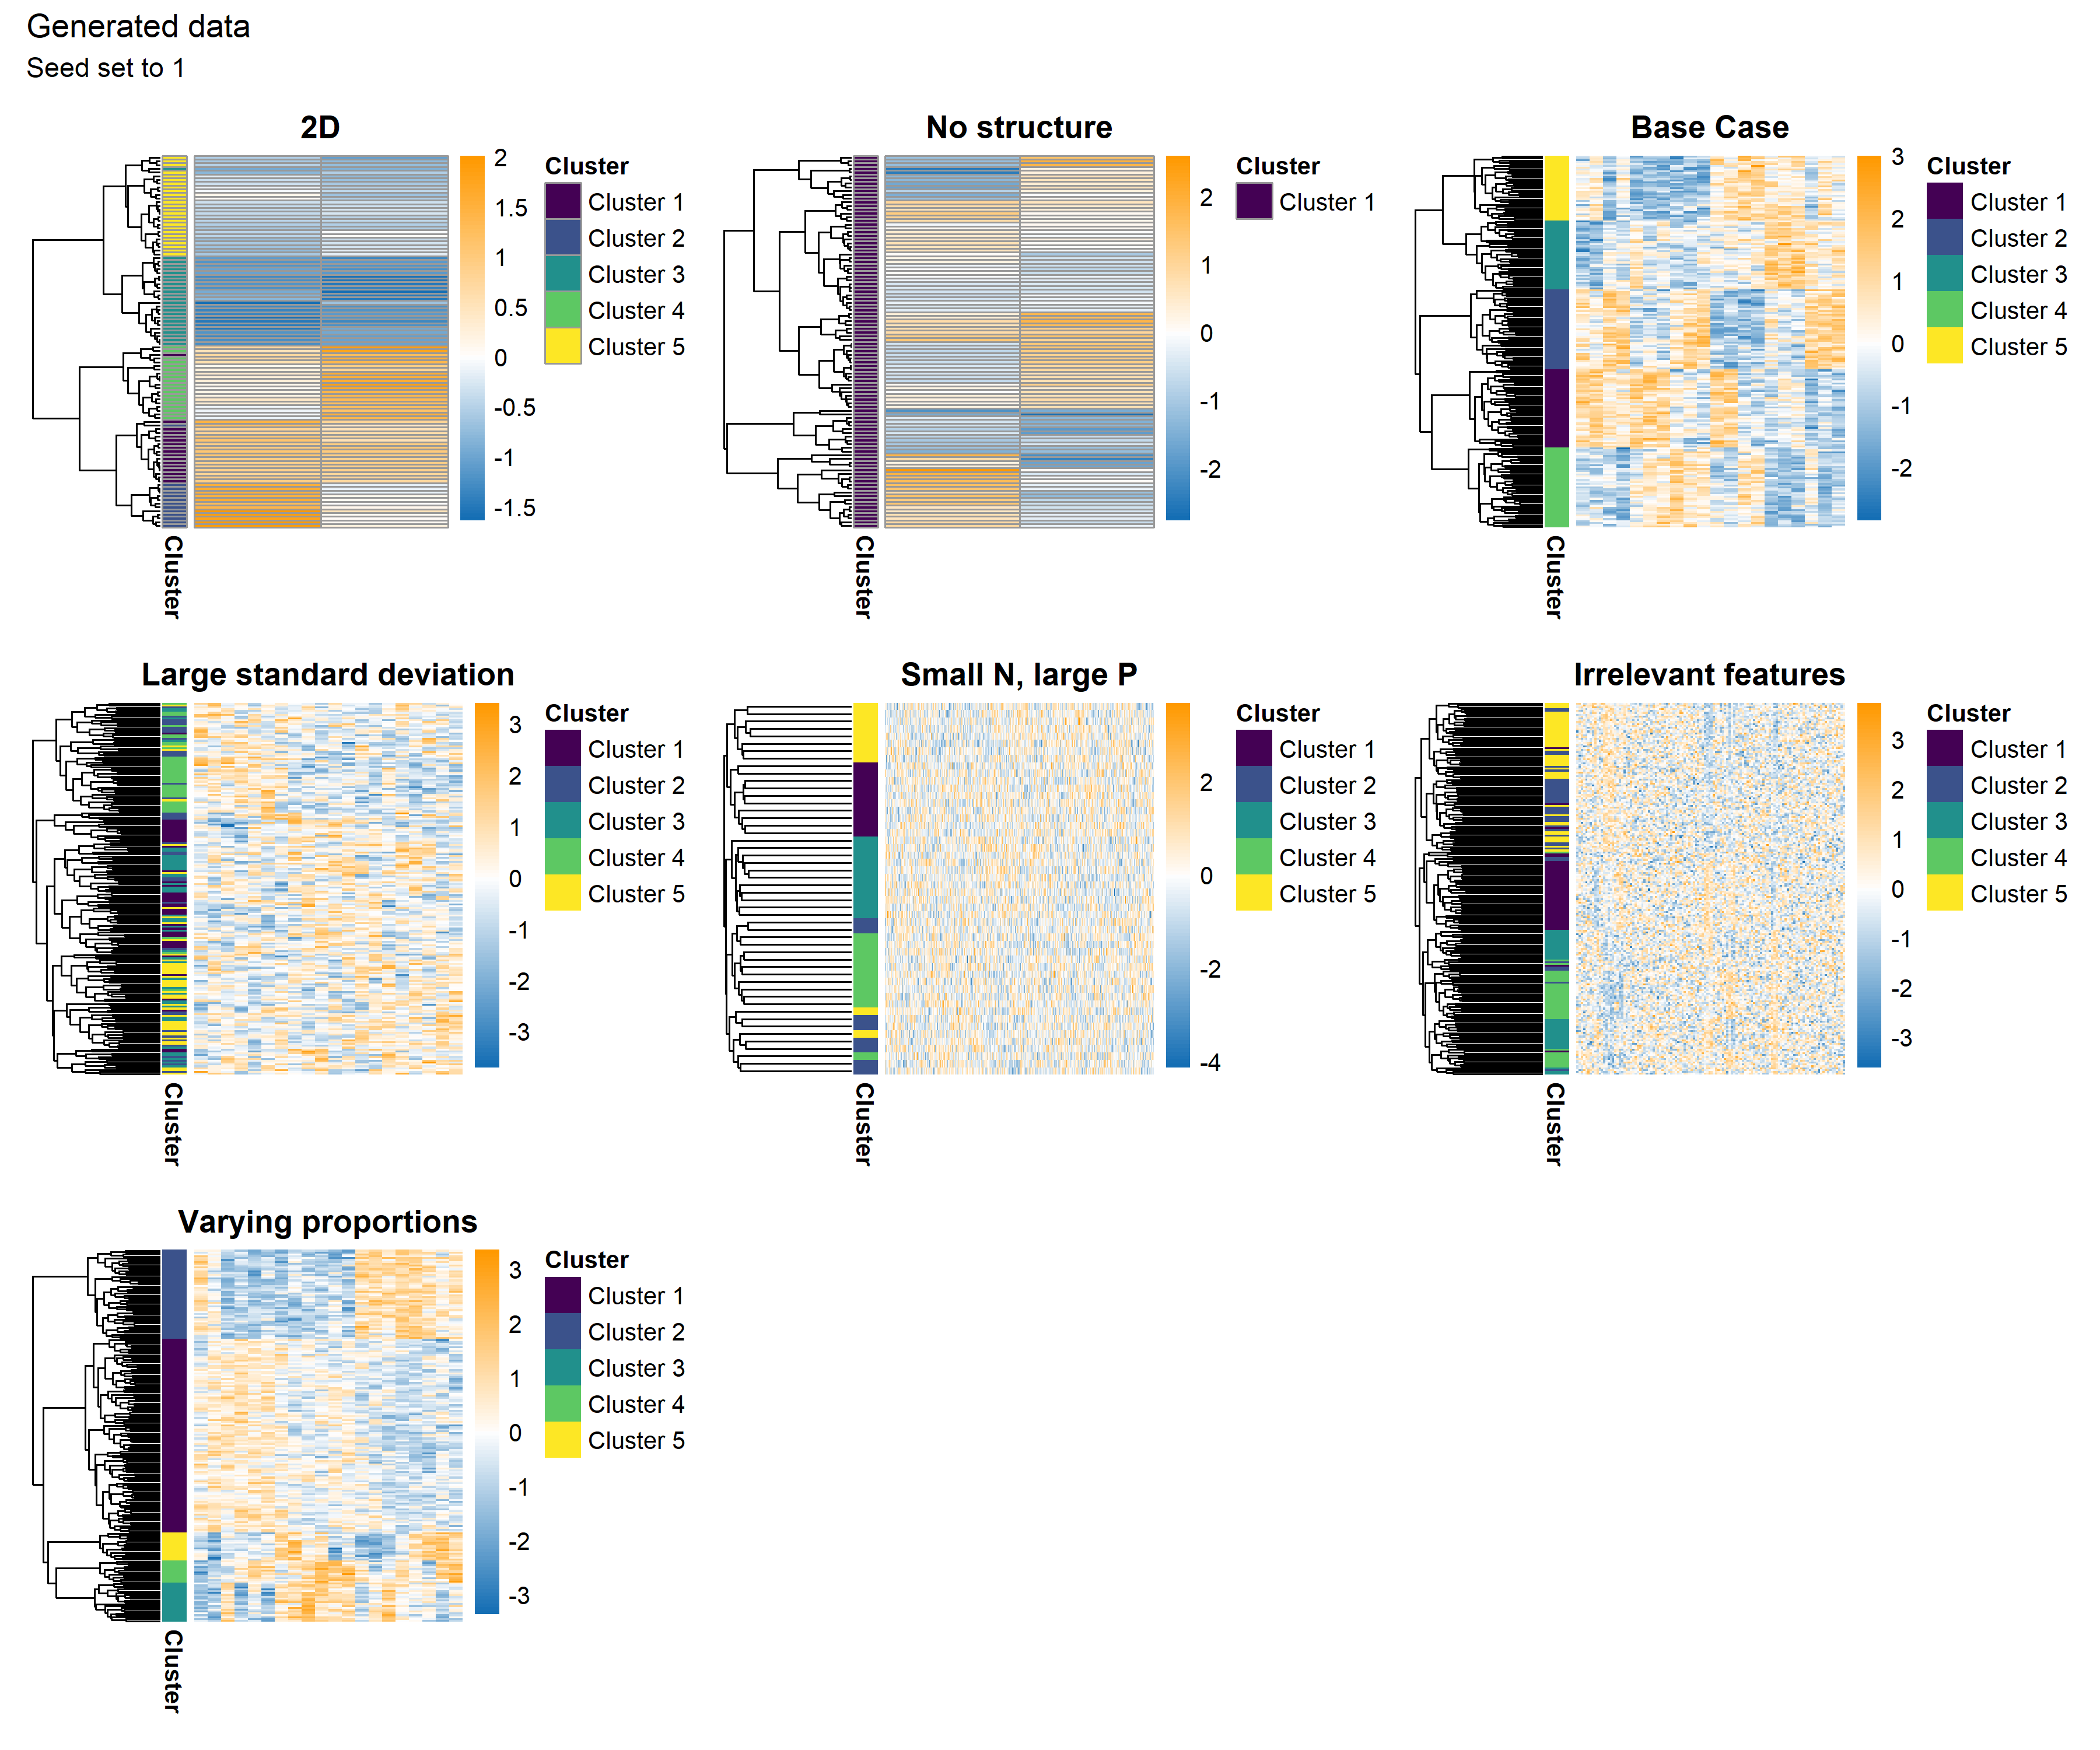
\includegraphics{./Images/Simulations/generated_datasets.png}
%	\caption{Example of generated datasets for different scenarios.}
%	\label{fig:genData}
%\end{sidewaysfigure}


%	\begin{sidewaysfigure}
%		\centering
%		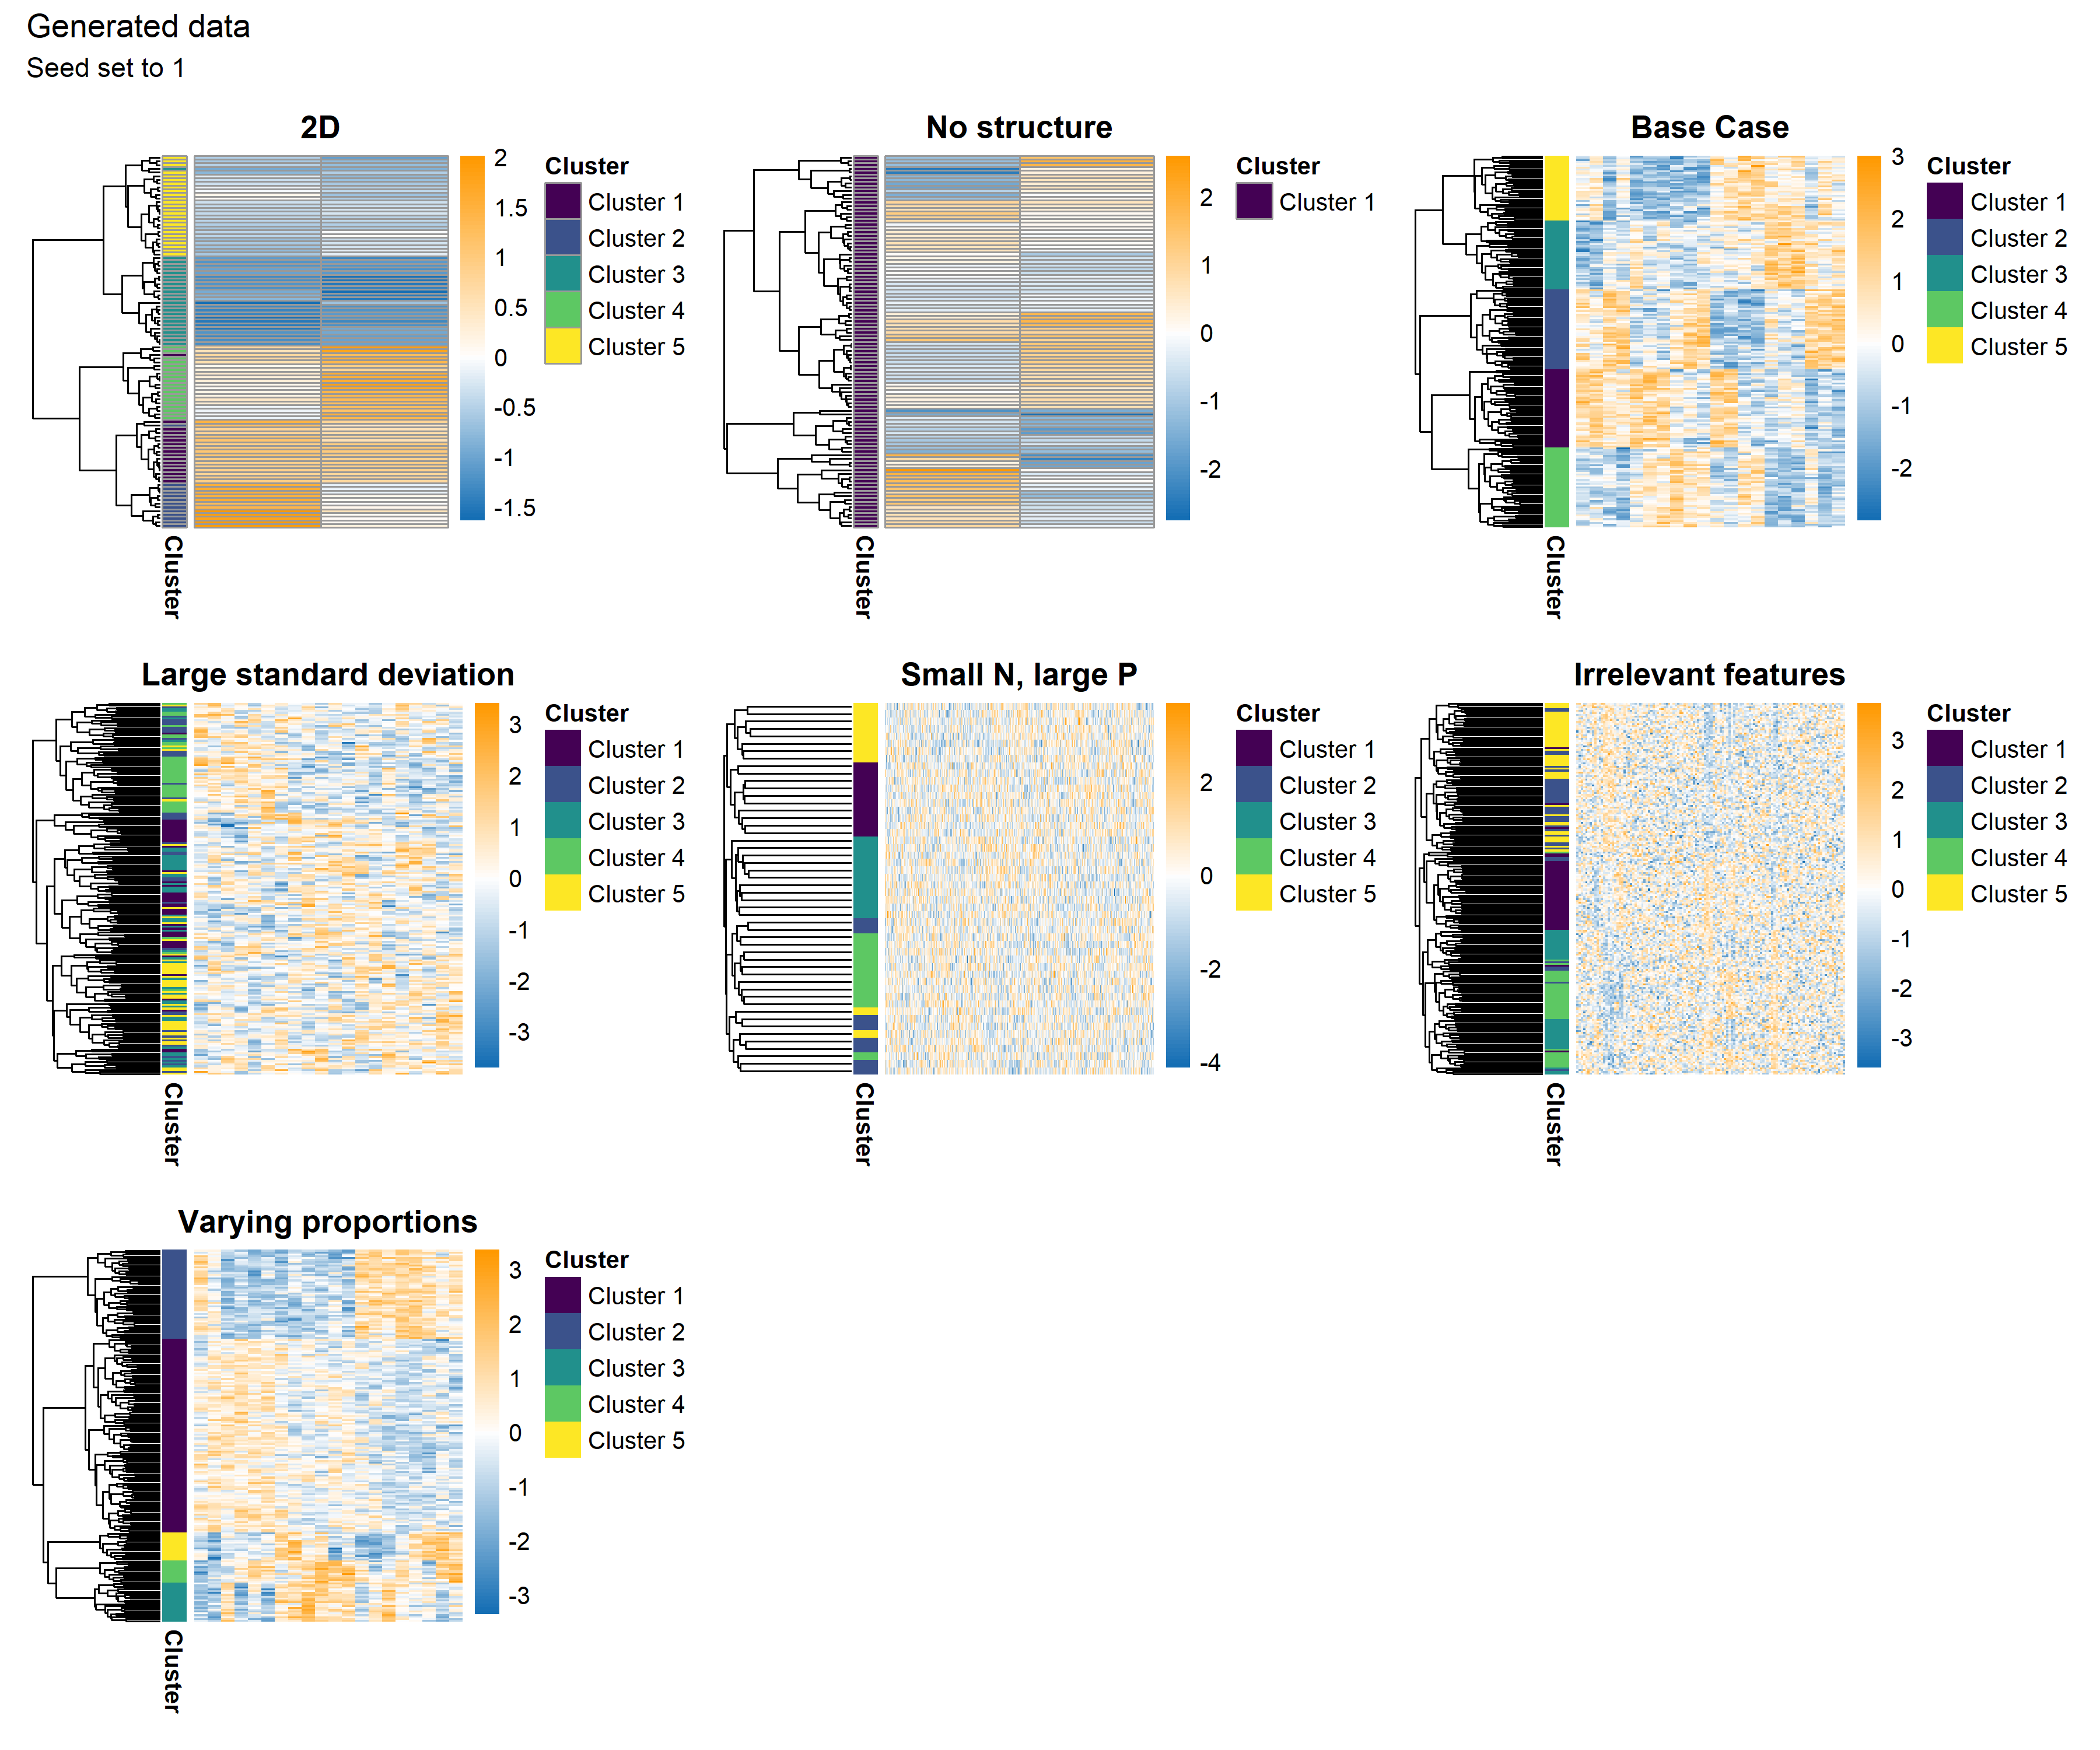
\includegraphics[scale=0.75]{./Images/Simulations/generated_datasets.png}
%		\caption{Example of generated datasets for different scenarios.}
%		\label{fig:genData}
%	\end{sidewaysfigure}


%\begin{tabular}{|l|ccccccc|}
%	\hline
%	\textbf{Scenario} & $N$ & $P_s$ & $P_n$ & $K$ & $\Delta_{\mu}$ & $\sigma^2$ & $\pi$\\
%	\hline 
%	Simple 2D & 100 & 2 & 0 & 5 & 3.0 & 1 &  $(\frac{1}{5} , \frac{1}{5}, \frac{1}{5}, \frac{1}{5}, \frac{1}{5})$ \\
%	%		\hline
%	No structure & 100 & 0 & 2 & 1 & 0.0 & 1 & 1 \\
%	%		\hline
%	Base Case & 200 & 20 & 0 & 5 & 1.0 & 1 &  $(\frac{1}{5} , \frac{1}{5}, \frac{1}{5}, \frac{1}{5}, \frac{1}{5})$\\
%	%		\hline
%	Large standard deviation & 200 & 20 & 0 & 5 & 1.0 & 3 & $(\frac{1}{5} , \frac{1}{5}, \frac{1}{5}, \frac{1}{5}, \frac{1}{5})$ \\
%	%		\hline
%	Large standard deviation & 200 & 20 & 0 & 5 & 1.0 & 5 &  $(\frac{1}{5} , \frac{1}{5}, \frac{1}{5}, \frac{1}{5}, \frac{1}{5})$\\
%	%		\hline
%	Irrelevant features & 200 & 20 & 10 & 5 & 1.0 & 1 &  $(\frac{1}{5} , \frac{1}{5}, \frac{1}{5}, \frac{1}{5}, \frac{1}{5})$\\
%	%		\hline
%	Irrelevant features & 200 & 20 & 20 & 5 & 1.0 & 1 &  $(\frac{1}{5} , \frac{1}{5}, \frac{1}{5}, \frac{1}{5}, \frac{1}{5})$\\
%	%		\hline
%	Irrelevant features & 200 & 20 & 100 & 5 & 1.0 & 1 &  $(\frac{1}{5} , \frac{1}{5}, \frac{1}{5}, \frac{1}{5}, \frac{1}{5})$\\
%	%		\hline
%	Varying proportions & 200 & 20 & 0 & 5 & 1.0 & 1 & $(\frac{1}{2} , \frac{1}{4}, \frac{1}{8}, \frac{1}{16}, \frac{1}{16})$ \\
%	Varying proportions & 200 & 20 & 0 & 5 & 0.4 & 1 &  $(\frac{1}{2} , \frac{1}{4}, \frac{1}{8}, \frac{1}{16}, \frac{1}{16})$ \\ %(0.5, 0.25, 0.125, 0.0675, 0.0675)\\
%	%		\hline
%	Small N, large P & 50 & 500 & 0 & 5 & 1.0 & 1 &  $(\frac{1}{5} , \frac{1}{5}, \frac{1}{5}, \frac{1}{5}, \frac{1}{5})$\\
%	%		\hline
%	Small N, large P & 50 & 500 & 0 & 5 & 0.2 & 1 &  $(\frac{1}{5} , \frac{1}{5}, \frac{1}{5}, \frac{1}{5}, \frac{1}{5})$
%%	\\
%%	\hline
%%	\caption{Parameters defining the simulation scenarios as used in generating data and labels.}
%	\label{table:scenarioTable}
%\end{tabular}

%Each scenario is seen as testing certain concepts or else specific characteristics of real data. An example of each scenario may be seen in figure \ref{fig:genData}.

\subsection{Performance quantification}

We use the Adjusted Rand Index as our metric for the quality of the point clustering inferred by each method, comparing this estimate with the generating labels produced by algorithm 1 in the supplementary materials.
% \ref{algorithm:simulationGeneration}. 
This is a measure of ``predictive performance'', the ability of the methods to infer a single partition that and its similarity to the truth. We also attempt to summarise the uncertainty quantification from each by computing the Frobenius Norm between the true coclustering matrix and the 

\begin{itemize}
	\item consensus matrix for consensus clustering,
	\item posterior similarity matrix for the Bayesian inference, and
	\item coclustering matric for \texttt{mclust}.
\end{itemize}
The Frobenius Norm will provide some information if the above matrices correspond at all to the true coclustering matrix, but if no method has performed well then this Norm will reward the \emph{singleton solution} wherein all items are allocated to individual clusters. This means that a visual inspection of  the PSMs and CMs is also required. As \texttt{mclust} provides only a point estimate the ARI between this and the truth will contain the required information.

The runtime of each MCMC chain is calculated using the terminal command \texttt{time}, measured in milliseconds.

\subsection{Bayesian model convergence}
To assess within-chain convergence of our Bayesian inference we use the Geweke $Z$-score statistic (\citealp{geweke1991evaluating}). Of the chains that appear to behave properly we then asses across-chain convergence using $\hat{R}$ (\citealp{gelman1992inference}) and the recent extension provided by \citealp{vats2018revisiting}. 

If a chain has reached its stationary distribution the Geweke statistic is expected to be normally distributed. Normality is tested for using a Shapiro-Wilks test (\citealp{shapiro1965analysis}). If a chain fails this test (i.e. the associated $p$-value is less than 0.05), we assume that is has not achieved stationarity and is excluded from the remainder of the analysis.

The Vats and Knudson extension of $\hat{R}$ is a summary statistic for the entire chain; this is the primary indicator of failure for convergence, but a visualisation of the original $\hat{R}$ diagnostic is also considered. 

\end{methods}

\section{Examples}

\subsection{Simulations}

\begin{figure}
	\centering
	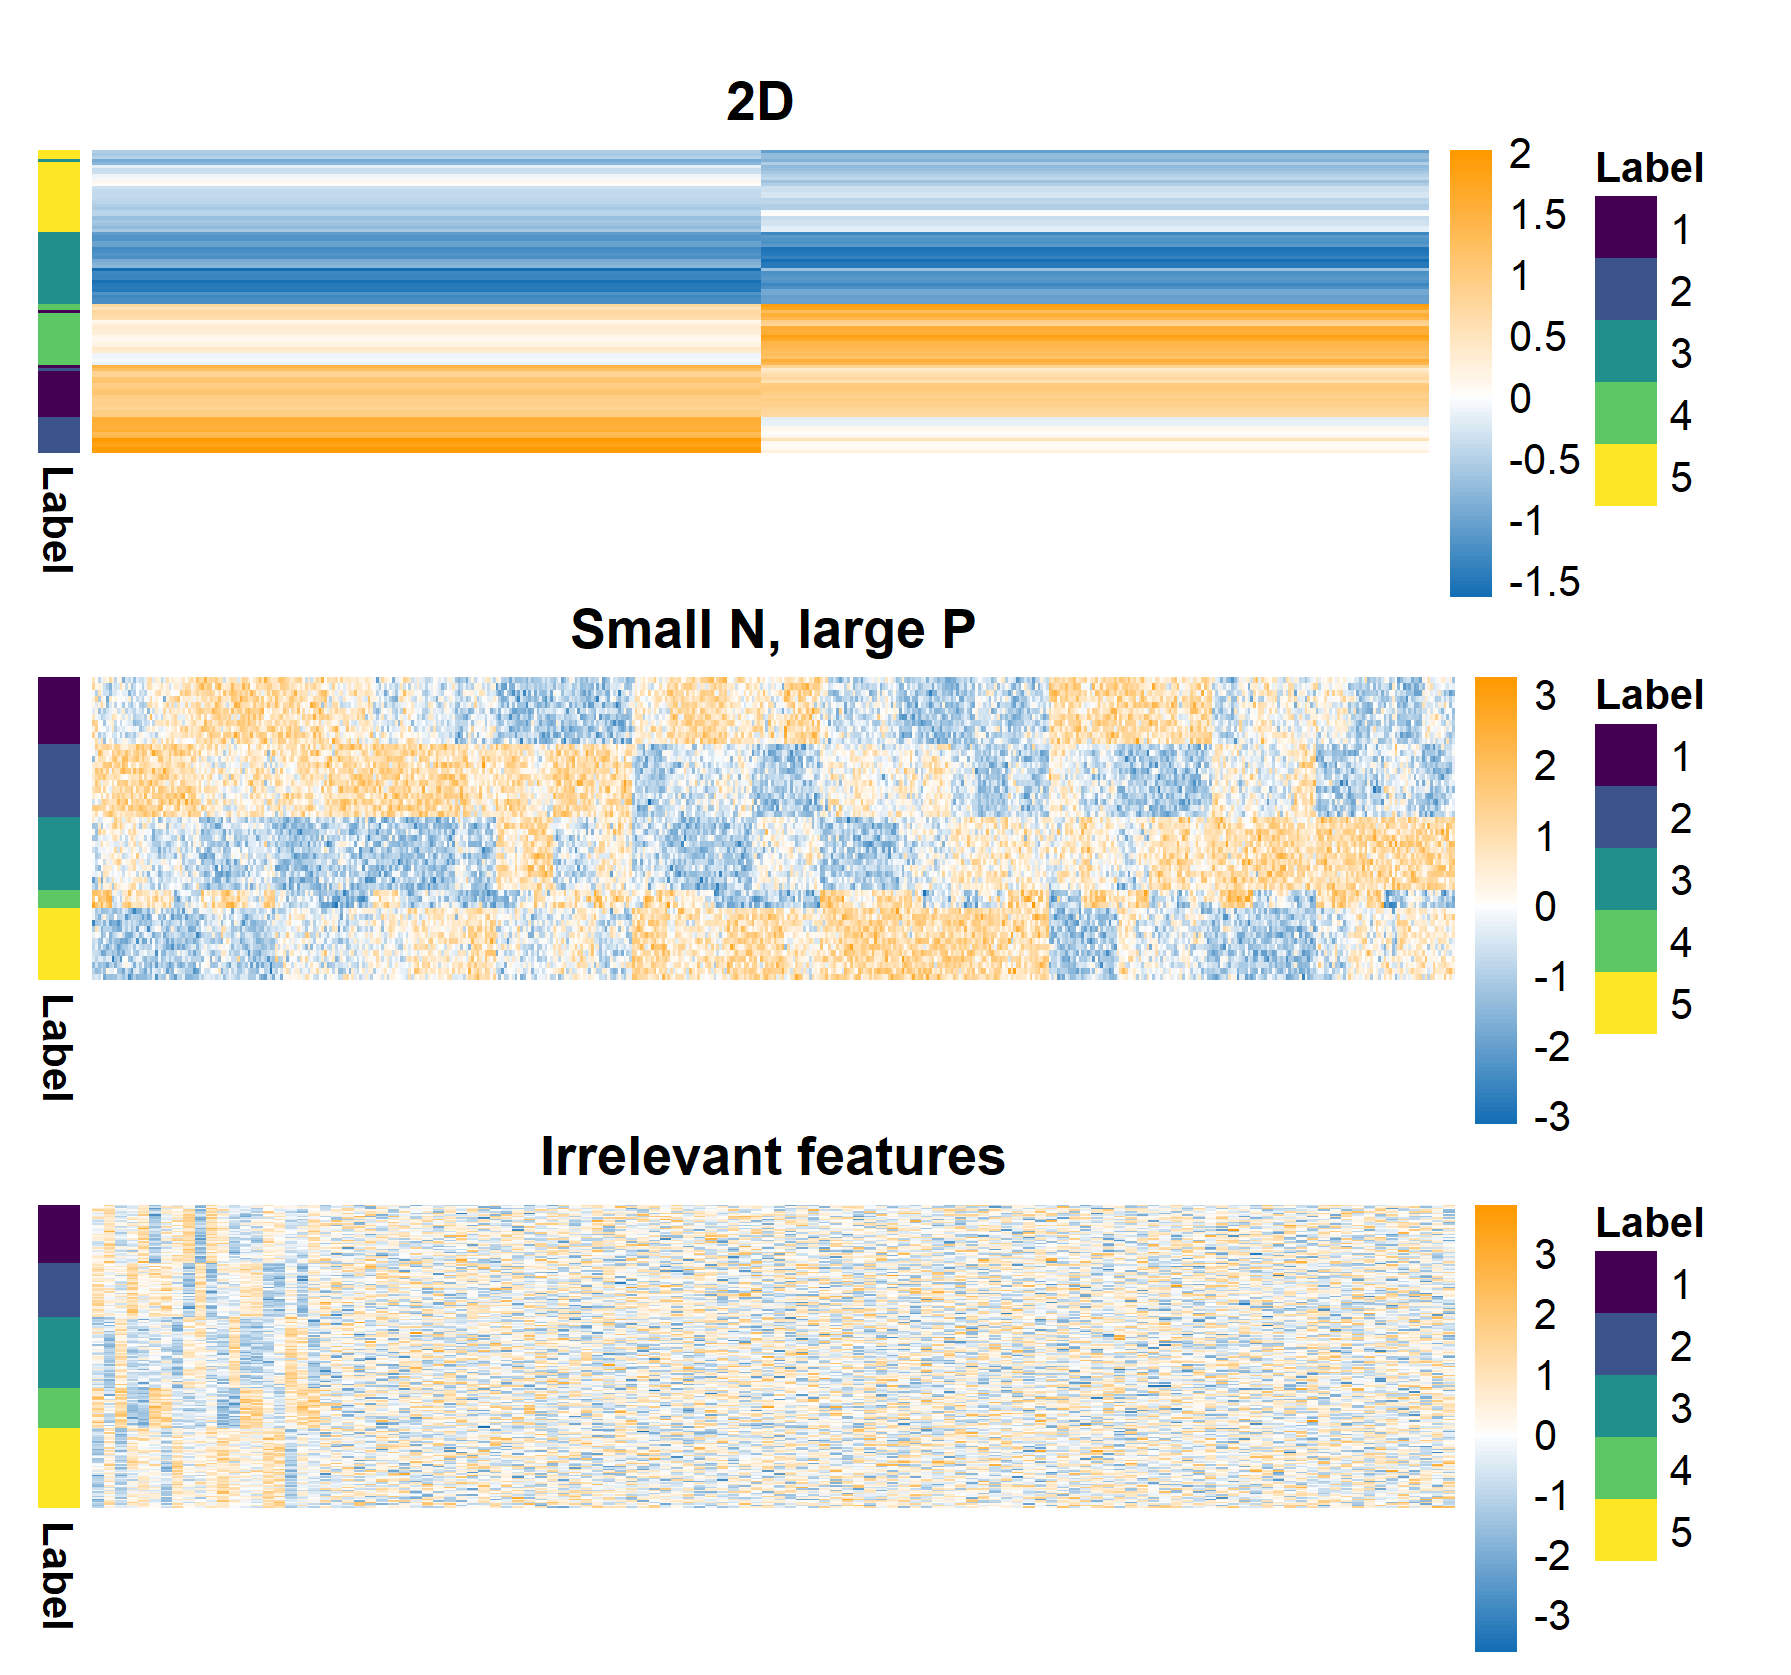
\includegraphics[scale=0.6]{./Images/Simulations/Data.png}
	\caption{Example of generated datasets. The low-dimensional dataset should enable proper mixing of chains in the MCMC and is less likely to have a local mode that traps \texttt{mclsut}. The small $N$, large $P$ case has clear structure (observable by eye). This is intended to highlight the problems of poor mixing due to high dimensions even when the generating labels are quite identifiable. In the irrelevant features case the structure is clear in the relevant features (on the lefthand side of this heatmap). This setting is intended to test how sensitive each approach is to noise.}
	\label{fig:genData}
\end{figure}

We compare consensus clustering of Bayesian mixture models to a traditional inference using several long chains of 1 million iterations (thinning to every thousandth) and an maximum-likelihood estimator as implement in the R package \texttt{mclust} \citealp{mclust2016scrucca}. These are compared within a range of simulations described in table \ref{table:scenarioTable}. In this article we describe the results of three of these in more detail with the remainder described in the supplementary material.

We test different scenarios that change various parameters in this model. The scenarios tested and there defining parameters are shown in table \ref{table:scenarioTable}. In this case the number of relevant features (\(P_s\)) is $\sum_p \phi_p$, and $P_n = P - P_s$.

\begin{table}[ht]
	\centering
	\caption{Parameters defining the simulation scenarios as used in generating data and labels. Results for the \emph{Simple 2D}, the first \emph{Small N, large P} and final \emph{Irrelevant features} scenarios are shown in this report, please see the supplementary material for additional results. The number of relevant features (\(P_s\)) is $\sum_p \phi_p$, and $P_n = P - P_s$.}
	\begin{tabular}{l|ccccccc}
		\toprule
		\textbf{Scenario} & $N$ & $P_s$ & $P_n$ & $K$ & $\Delta_{\mu}$ & $\sigma^2$ & $\pi$\\
		\midrule
		2D & 100 & 2 & 0 & 5 & 3.0 & 1 &  $(\frac{1}{5} , \frac{1}{5}, \frac{1}{5}, \frac{1}{5}, \frac{1}{5})$ \\
		%		\hline
%		No structure & 100 & 0 & 2 & 1 & 0.0 & 1 & 1 \\
%		%		\hline
%		Base Case & 200 & 20 & 0 & 5 & 1.0 & 1 &  $(\frac{1}{5} , \frac{1}{5}, \frac{1}{5}, \frac{1}{5}, \frac{1}{5})$\\
%		%		\hline
%		Standard deviation & 200 & 20 & 0 & 5 & 1.0 & 3 & $(\frac{1}{5} , \frac{1}{5}, \frac{1}{5}, \frac{1}{5}, \frac{1}{5})$ \\
%		%		\hline
%		Standard deviation & 200 & 20 & 0 & 5 & 1.0 & 5 &  $(\frac{1}{5} , \frac{1}{5}, \frac{1}{5}, \frac{1}{5}, \frac{1}{5})$\\
%		%		\hline
%		Irrelevant features & 200 & 20 & 10 & 5 & 1.0 & 1 &  $(\frac{1}{5} , \frac{1}{5}, \frac{1}{5}, \frac{1}{5}, \frac{1}{5})$\\
%		%		\hline
%		Irrelevant features & 200 & 20 & 20 & 5 & 1.0 & 1 &  $(\frac{1}{5} , \frac{1}{5}, \frac{1}{5}, \frac{1}{5}, \frac{1}{5})$\\
%		%		\hline
		Irrelevant features & 200 & 20 & 100 & 5 & 1.0 & 1 &  $(\frac{1}{5} , \frac{1}{5}, \frac{1}{5}, \frac{1}{5}, \frac{1}{5})$\\
		%		\hline
%		Varying proportions & 200 & 20 & 0 & 5 & 1.0 & 1 & $(\frac{1}{2} , \frac{1}{4}, \frac{1}{8}, \frac{1}{16}, \frac{1}{16})$ \\
%		Varying proportions & 200 & 20 & 0 & 5 & 0.4 & 1 &  $(\frac{1}{2} , \frac{1}{4}, \frac{1}{8}, \frac{1}{16}, \frac{1}{16})$ \\ %(0.5, 0.25, 0.125, 0.0675, 0.0675)\\
%		%		\hline
		Small N, large P & 50 & 500 & 0 & 5 & 1.0 & 1 &  $(\frac{1}{5} , \frac{1}{5}, \frac{1}{5}, \frac{1}{5}, \frac{1}{5})$\\
		%		\hline
%		Small N, large P & 50 & 500 & 0 & 5 & 0.2 & 1 &  $(\frac{1}{5} , \frac{1}{5}, \frac{1}{5}, \frac{1}{5}, \frac{1}{5})$
		%	\\
		%	\hline
%		\\
		\botrule
	\end{tabular}
	\caption{Parameters defining the simulation scenarios as used in generating data and labels.}
	\label{table:scenarioTable}
\end{table}%

The examples included in this article are
\begin{itemize}
	\item a low-dimensional dataset,
	\item a wide dataset representative of the \emph{small $N$, large $P$} paradigm prevalent in genetics, and
	\item a dataset with a large number of irrelevant features.
\end{itemize}
The first of these is expected to be the setting where \texttt{mclust} and the individual long chains behave well. In the other simulations increasing dimensionality means that mixing problems can emerge and the chains become liable to being trapped in individual modes. Within each simulation 100 datasets are generated following algorithm \ref{algorithm:simulationGeneration}. To each of these datasets 

\begin{itemize}
	\item \texttt{mclust} (for a range of possible $K$),
	\item 10 chains of 1 million iterations, thinning to every thousandth sample for the overfitted Bayesian mixture model, and
	\item a variety of consensus clustering ensembles defined by inputs of $S$ chains and $R$ iterations within each chain (see algorithm \ref{algorithm:CCforBayesianMixtures}) with $S \in \{1, 10, 30, 50, 100\}$ and $R \in \{1, 10, 100, 1000, 10000\}$,
\end{itemize}
are applied. In theory we would expect the Bayesian chains to explore a common posterior distribution, but the practice sees chains become trapped in distinct modes in different scenarios. We believe that the mode within which the greatest number of chains become trapped would be that which is used to perform the inference in a real application (and longer chains did not solve the problem). As part of a pipeline where such analyses have to happen $12 \times 100 = 1,200$ times, we pool the Bayesian samples into a single PSM as manually assessing which mode is dominant. As visual inspection of the PSMs indicates that the disagreement between modes tends to be one of 
\begin{itemize}
	\item several clusters are merged or
	\item a cluster is represented by two or more components,
\end{itemize}
each of the modes tends to have large overlap with all others. This means that the clustering inferred from the PSM created from the samples pooled across all stationary chains will represent the most popular mode and the ARI will not be unduly inflated. The Frobenius norm between the PSM and the true coclustering will be less representative of a single chain as more modes will be represented and therefore greater uncertainty than any single chain. This is inline with our previous assertion that the Frobenius statistic is more an indicator that should be used along with visual assessment of examples of the PSMs and CMs from a simulation rather than sufficiently informative in and of itself.



%Multiple dataset
%\begin{itemize}
%	\item MDI yeast
%	\item BCC?
%	\item PanCancer data\vspace*{1pt}
%\end{itemize}


\section{Results}
\subsection{Simulations}
A summary of the results for a selection of the simulation scenarios are shown in table \ref{table:meanARISims} and figure \ref{fig:simResults}. In the strong signal scenarios (i.e. noise free and clearly distinguishable generating clusters), \texttt{mclust} performs very well, correctly identifying the true structure However, a large number of irrelevant features completely erodes the ability of \texttt{mclust} to uncover meaningful structure. The pooled samples from multiple long chains performs consistently very well. This is not surprising as the pooling effect means that any multi-modality present in the data does not present any degree of problem. In this case the pooled samples, themselves a consensus of 10 models, acts as an upper bound on the more practical implementations of consensus clustering. Consensus clustering does consistently uncover structure in the data. With sufficiently large ensembles and chain depth, consensus clustering is close to the pooled Bayesian samples in predictive performance. In terms of the Frobenius norm, many of the consensus clustering results have significant overlap with the pooled long chains.

\begin{table}[ht]
	\centering
	\caption{Mean ARI for 100 datasets within three simulation scenarios between the generating labels and the predicted clustering for a subset of methods. CC($r, s$) indicates consensus clustering using the $r^{th}$ sample from $s$ chains.}
	\begin{tabular}{l|rrr}
		\toprule
		\textbf{Model} & 2D & Small $N$, large $P$ & Irrelevant features \\
		\midrule
		Mclust & 0.970 &       1.000 &         0.000\\
		Bayesian (Pooled) &  0.669 & 				0.999 &         0.946\\
		CC(10, 10) & 0.362 &	            0.997 &         0.385\\
		CC(100, 10) & 0.844 &			    0.346 &         0.999\\
		CC(100, 50) & 0.873 &			    0.517 &         0.999\\
		CC(100, 100) & 0.879 &  			0.576 &         0.999\\
		CC(10000, 10) & 0.348 &             0.999 &			0.935\\
		CC(10000, 100) & 0.570 &            0.999 &			0.944\\
		\botrule
	\end{tabular}
	\label{table:meanARISims}
\end{table}
It can be seen from table \ref{table:meanARISims} and figures \ref{fig:simResults} that 

\begin{figure} %[!tpb]
	\centering
	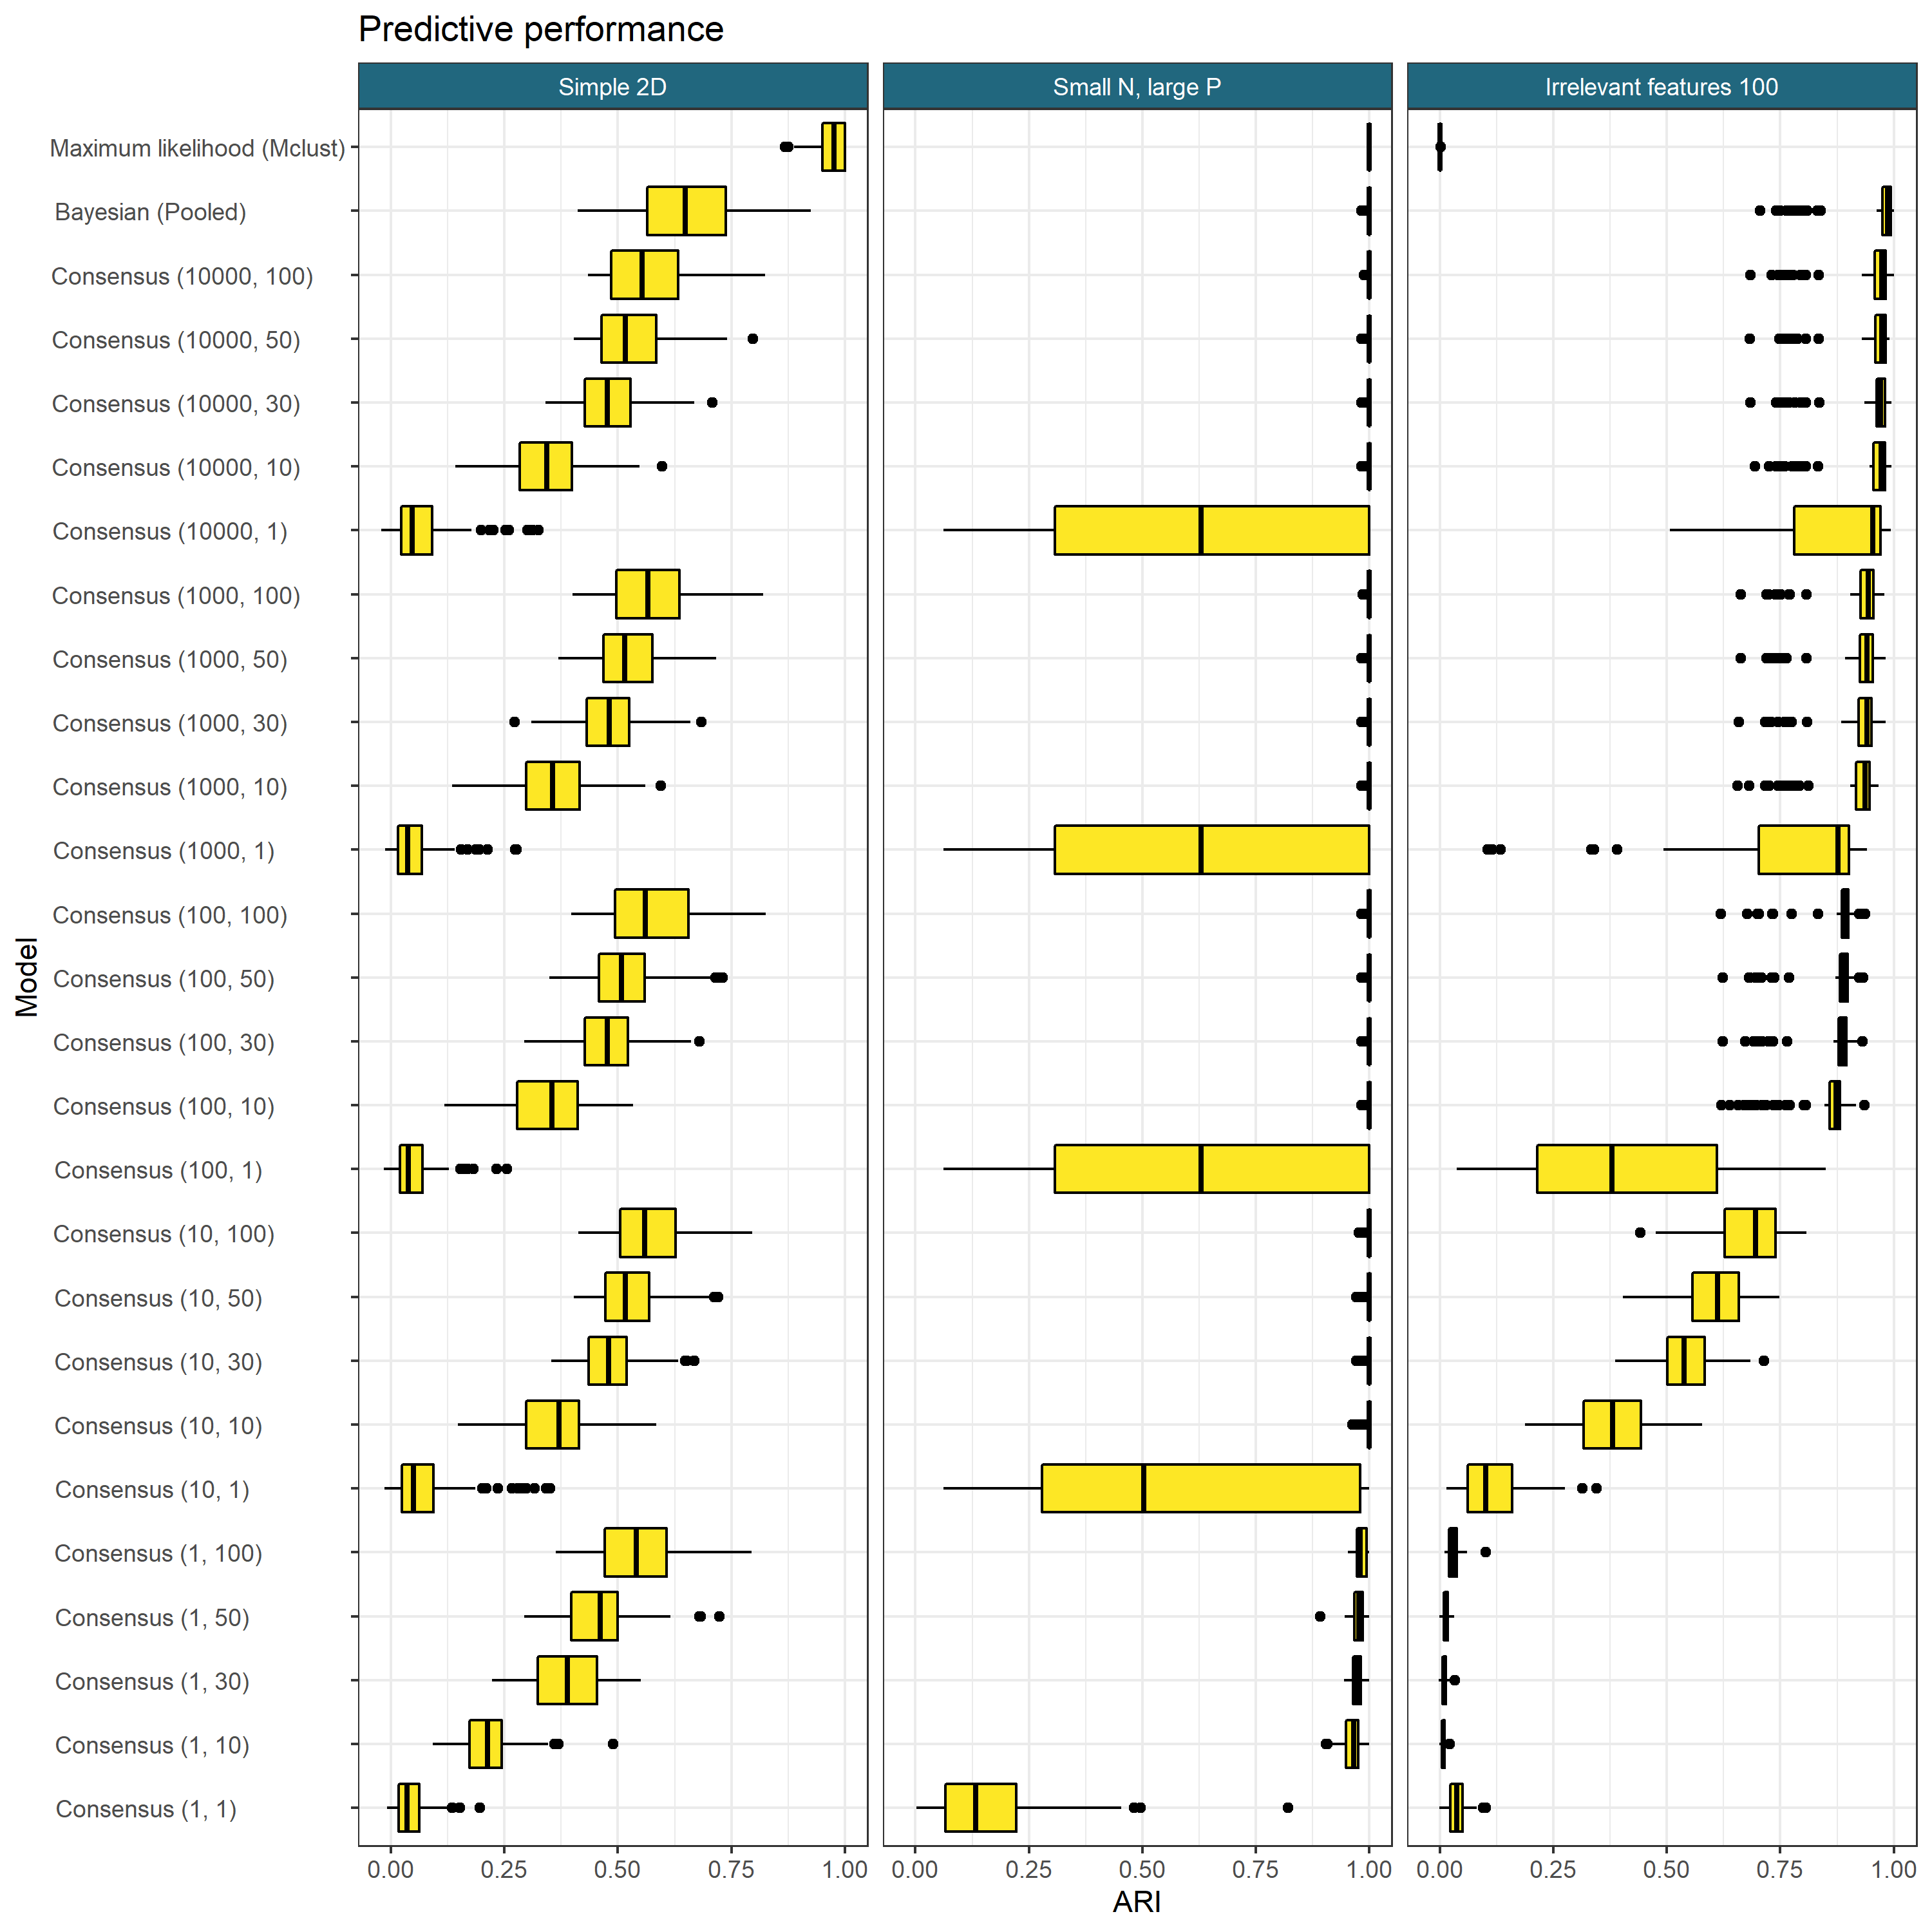
\includegraphics[scale=0.5]{./Images/Simulations/simulation_model_prediction.png}
	\caption{Model performance in a subset of simulation scenarios. }
	\label{fig:simResults}
\end{figure}

\begin{figure} %[!tpb]
	\centering
	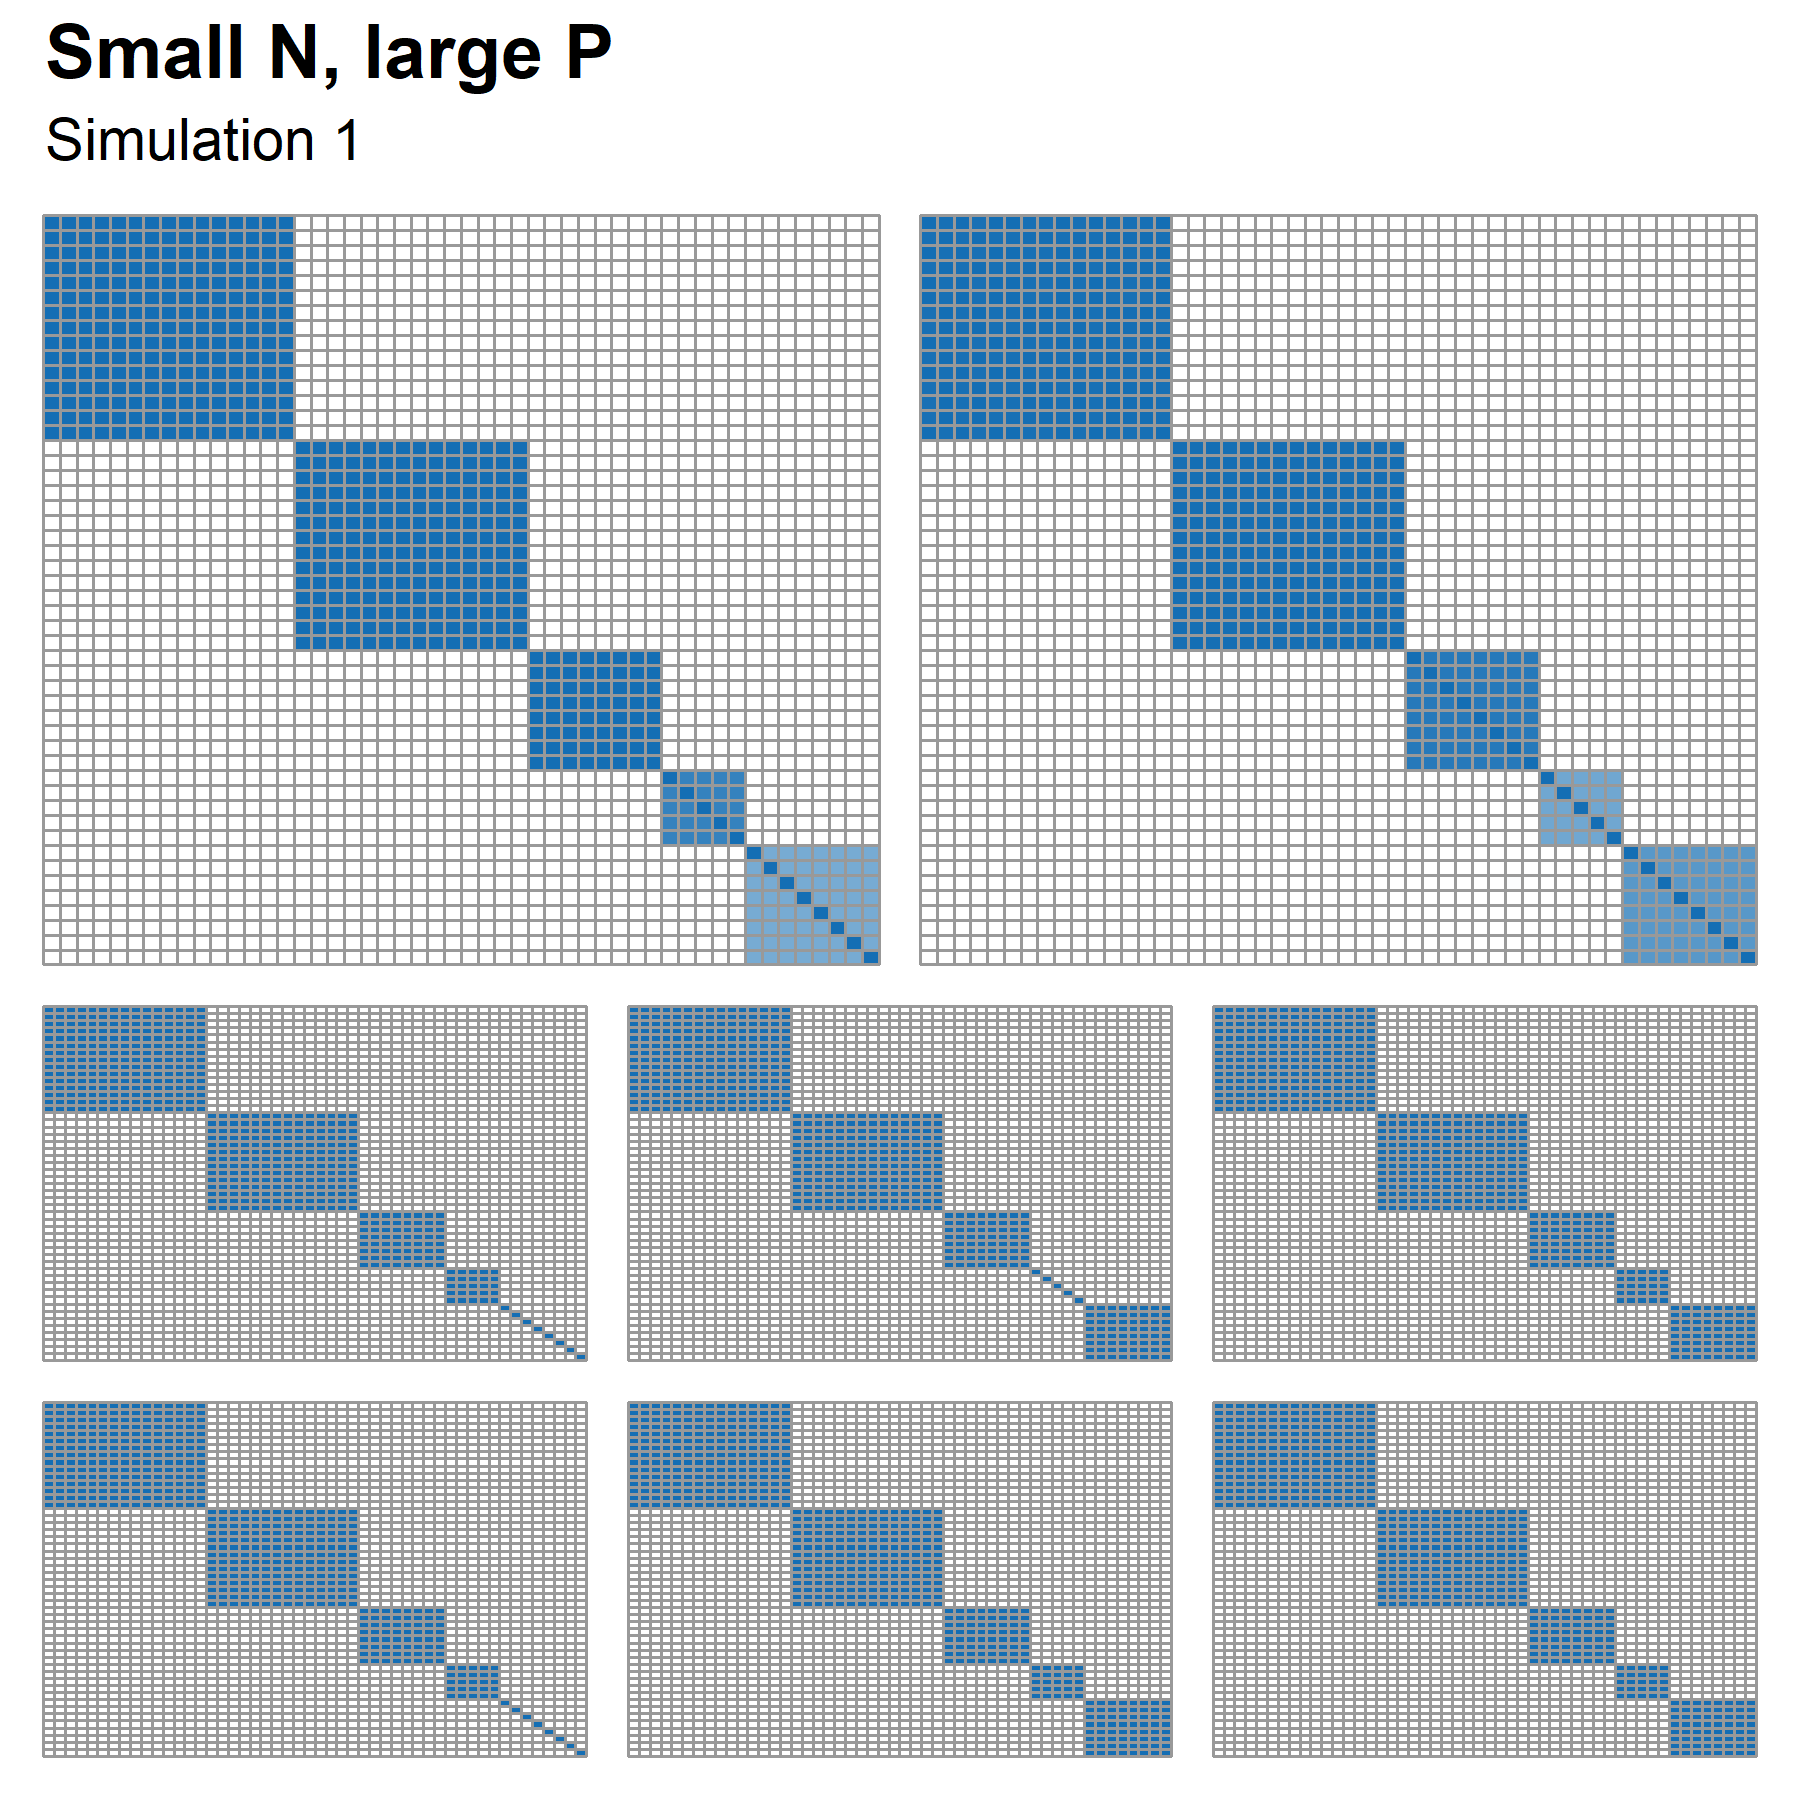
\includegraphics[scale=0.5]{./Images/Simulations/small_n_large_p_base/comp_psms_cm.png}	
%PSMs/BayesianSimulation2PSMs.png}
%	\caption{PSMs for 8 chains that pass within chain convergence test. Rows and columns are ordered by a hierarchical clustering applied to the matrix in the bottom right. Annotations are the generating labels. The top row of PSMs are all in a common mode where Cluster 3 does not merge instead remaining as singletons. In the bottom row the first, second and fourth matrices correctly cluster all 5 clusters. The third matrix uncovers a different mode where Cluster 5 does not merge. The matrices appear binary, suggesting no diversity in the partitions being sampled.}
	\caption{In the first row the PSM of the pooled Bayesian samples is compared to the CM for CC(100, 50), with a common ordering of rows and columns in both heatmaps. There is very little difference between these two objects. In the next two rows the PSMs constructed from 6 of the long chains that passed the stationarity test are displayed. Three different modes emerge across the different chains.}
	\label{fig:simSmallNLargePPSMs}
\end{figure}

Figure \ref{fig:simSmallNLargePPSMs} shows an example of different chains becoming trapped in different modes and failing to explore a common partition space. In the simulations shown here the overlap between the modes and signal in the data is clear enough that one can pick the true clustering structure and select the chain that best represents this, but in other

\begin{figure} %[!tpb]
	\centering
	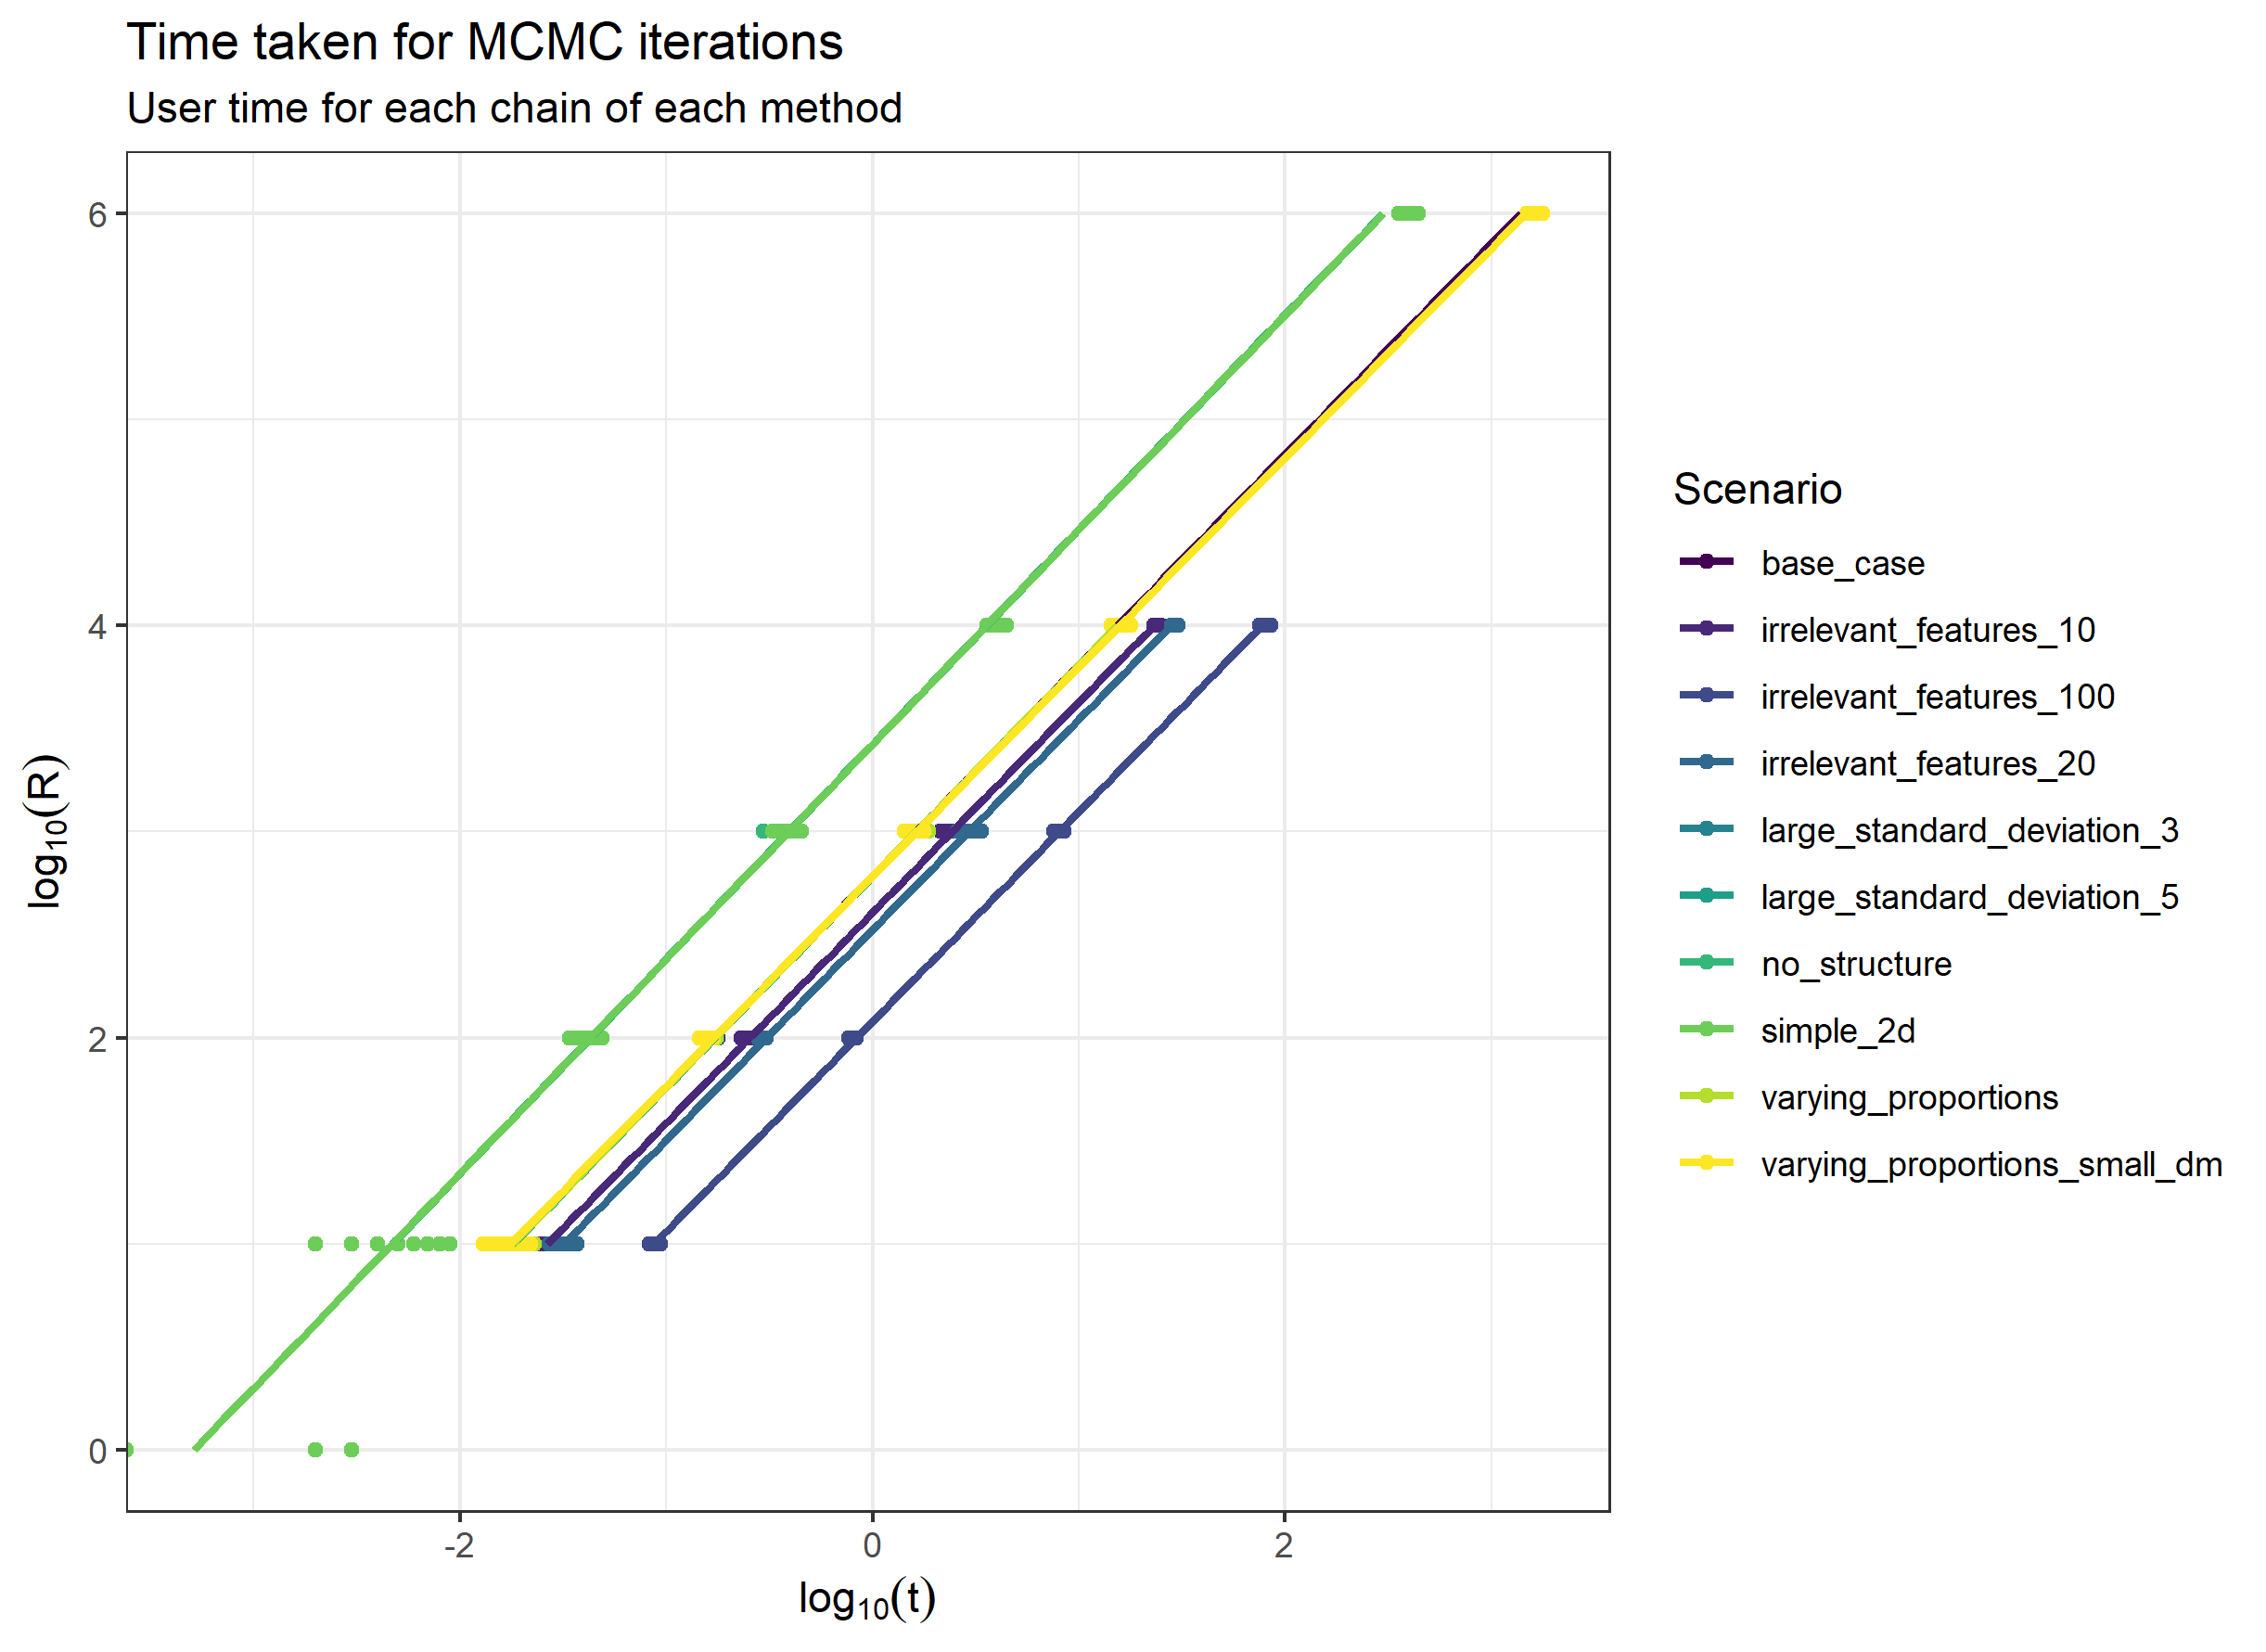
\includegraphics[scale=0.5]{./Images/Simulations/TimeComparison.png}	
	\caption{The time taken for different numbers of iterations of MCMC moves. The relationship between chain length, $R$, and the time taken is linear, with a change of intercept for different dimensions.}
	\label{fig:timeMCMC}
\end{figure}

Figure \ref{fig:timeMCMC} reveals the gains in computation runtime achieved by consensus clustering when a parallel environment is available. If a single iteration requires $t$ seconds, running 100 chains of length 100 using 8 cores takes $1,300t$ compared to 5 chains of 10,000 iterations taking $10,000t$. 

%In the 2D dataset \texttt{mclust} outperforms the Bayesian inference and consensus clustering in terms of the point estimate of the generating structure. 

%\begin{itemize}
%	\item Simple example - Mclust and Bayesian win! We see MCMC exploring well. 
%	\item Small N large P, problems for Bayesian. Separate modes represented in CM, so consensus is finding sensible modes
%	\item Irrelevant 100, many modes, Mclust collapse, similar to above.
%	\item Real data \vspace*{1pt}
%\end{itemize}
%
%Multiple dataset
%\begin{itemize}
%	\item MDI yeast - pretty identical
%	\item Full yeast - Bayesian fails, consensus succeeds
%	\item Cancer - hmmmmmm	\vspace*{1pt}
%\end{itemize}
%
%\begin{figure}[!tpb]%figure1
%\fboxsep=0pt\colorbox{gray}{\begin{minipage}[t]{235pt} \vbox to 100pt{\vfill\hbox to
%235pt{\hfill\fontsize{24pt}{24pt}\selectfont FPO\hfill}\vfill}
%\end{minipage}}
%%\centerline{\includegraphics{fig01.eps}}
%\caption{Caption, caption.}\label{fig:01}
%\end{figure}

%\begin{figure}[!tpb]%figure2
%%\centerline{\includegraphics{fig02.eps}}
%\caption{Caption, caption.}\label{fig:02}
%\end{figure}


%\subsection{Test1}


\section{Discussion}

In this article, we have extended Consensus clustering to Bayesian mixture models. This overcomes the problem of mixing for MCMC based clustering methods and also improves the speed at which an analysis can be performed. The proposed method has demonstrated good performance on simulation studies, having similar ability to uncover structure as more traditional approaches. It has better ability to represent several modes in the data than individual chains and is significantly faster, while retaining the ability to infer $K$, the number of occupied components present. 

We expect that our method will be useful to researchers analysing high-dimensional data where the runtime of MCMC methods becomes too onerous and multi-modality is more likely to be present.

Could the early stopping of the MCMC algorithm be a form of regularisation, making the model more robust to misspecification? In line with early stopping from Deep Learning (see \citealp{morgan1990generalization}), regularisation and misspecification idea from \cite{miller2018robust, cai2020finite}.


%%%%%%%%%%%%%%%%%%%%%%%%%%%%%%%%%%%%%%%%%%%%%%%%%%%%%%%%%%%%%%%%%%%%%%%%%%%%%%%%%%%%%
%
%     please remove the " % " symbol from \centerline{\includegraphics{fig01.eps}}
%     as it may ignore the figures.
%
%%%%%%%%%%%%%%%%%%%%%%%%%%%%%%%%%%%%%%%%%%%%%%%%%%%%%%%%%%%%%%%%%%%%%%%%%%%%%%%%%%%%%%






\section{Conclusion}

(Table~\ref{Tab:01}) Text Text Text Text Text Text  Text Text Text

\begin{enumerate}
\item this is item, use enumerate
\item this is item, use enumerate
\item this is item, use enumerate
\end{enumerate}




\section*{Acknowledgements}

Text Text Text Text Text Text  Text Text. nt to know about  text
text text text\vspace*{-12pt}

\section*{Funding}

This work has been supported by the... Text Text  Text Text.\vspace*{-12pt}

\bibliographystyle{natbib}
%\bibliographystyle{achemnat}
%\bibliographystyle{plainnat}
%\bibliographystyle{abbrv}
%\bibliographystyle{bioinformatics}
%
%\bibliographystyle{plain}
%
%\bibliography{document}
\bibliography{CCbib}  

% \begin{thebibliography}{}

% \bibitem[Bofelli {\it et~al}., 2000]{Boffelli03}
% Bofelli,F., Name2, Name3 (2003) Article title, {\it Journal Name}, {\bf 199}, 133-154.

% \bibitem[Bag {\it et~al}., 2001]{Bag01}
% Bag,M., Name2, Name3 (2001) Article title, {\it Journal Name}, {\bf 99}, 33-54.

% \bibitem[Yoo \textit{et~al}., 2003]{Yoo03}
% Yoo,M.S. \textit{et~al}. (2003) Oxidative stress regulated genes
% in nigral dopaminergic neurnol cell: correlation with the known
% pathology in Parkinson's disease. \textit{Brain Res. Mol. Brain
% Res.}, \textbf{110}(Suppl. 1), 76--84.

% \bibitem[Lehmann, 1986]{Leh86}
% Lehmann,E.L. (1986) Chapter title. \textit{Book Title}. Vol.~1, 2nd edn. Springer-Verlag, New York.

% \bibitem[Crenshaw and Jones, 2003]{Cre03}
% Crenshaw, B.,III, and Jones, W.B.,Jr (2003) The future of clinical
% cancer management: one tumor, one chip. \textit{Bioinformatics},
% doi:10.1093/bioinformatics/btn000.

% \bibitem[Auhtor \textit{et~al}. (2000)]{Aut00}
% Auhtor,A.B. \textit{et~al}. (2000) Chapter title. In Smith, A.C.
% (ed.), \textit{Book Title}, 2nd edn. Publisher, Location, Vol. 1, pp.
% ???--???.

% \bibitem[Bardet, 1920]{Bar20}
% Bardet, G. (1920) Sur un syndrome d'obesite infantile avec
% polydactylie et retinite pigmentaire (contribution a l'etude des
% formes cliniques de l'obesite hypophysaire). PhD Thesis, name of
% institution, Paris, France.

% \end{thebibliography}
\end{document}
